\documentclass[letterpaper,twocolumn,10pt]{article}
\usepackage{usenix-2020-09}
\usepackage{capt-of}

\usepackage{booktabs}
\usepackage{multirow}
\usepackage{amsmath}
\let\Bbbk\relax
\usepackage{amssymb}
\usepackage{graphicx}
\usepackage{xcolor}
\usepackage{url}
\usepackage{listings}
\usepackage{tabularx}
\usepackage{makecell}
\usepackage{hyperref}
\usepackage{adjustbox}
\usepackage{array}
\usepackage{tikz}
\usetikzlibrary{positioning,trees}

\lstdefinestyle{shellstyle_bw}{
    language=bash,
    basicstyle=\ttfamily\scriptsize,
    keywordstyle=\bfseries,
    commentstyle=\itshape,
    breaklines=true,
    breakatwhitespace=true,
    columns=fullflexible,
    keepspaces=true,
    showstringspaces=false,
    frame=single,
    xleftmargin=1em,
    framexleftmargin=1em,
    captionpos=b
}



\graphicspath{{figures/}}


\begin{document}

\title{On the Limits of General-Purpose LLMs for Network Intrusion Detection with Packet Metadata and Session Context}

\author{{\rm Anonymous Submission}}
\date{}

\maketitle

\begin{abstract}
Recent work suggests LLMs can be used for network intrusion detection with near-perfect accuracy, but most published work relies either on large, detailed datasets such as raw bytes, TLS metadata, or rich flow-level features, both of which are impractical in real-world, noisy, large-scale environments. We test whether a general-purpose LLM adds value when restricted to scalable, payload-free metadata and complete sessions, bounded windows or packets per session. Using capture-disjoint train/validation/test manifests over 12 PCAP datasets, we perform repeated holdout under balanced and deployment-mode session evaluation with validation-only threshold selection. The primary session suite evaluates OpenAI GPT-5.4 against classical ML and tree ensembles (RF, XGB, LGBM, CART, and KNN); the complementary packet archive additionally includes Anthropic Claude Sonnet 4.6 and classical LR, LDA, NB, SVC, and MLP. We utilize minimal (side-channel), Cisco Mercury-style, and combined traffic metadata over 150 local summaries and 30 LLM variants that cover sessions, windows, packets, and blind/training-memory prompts. The best balanced network session/window result is LGBM on 30-second windows ($F_1=84.28\%$), versus $66.83\%$ for GPT-5.4 on blind five-second windows. Local LGBM reaches $F_1=79.17\%$, when the best session LLM reaches only $57.25\%$ with 91.59\% recall but 55.36\% specificity. Local inference is approximately $0.003$ ms/sample, compared with $1.5$ s per remote call. A second cluster of packet-only experiments also reaffirms these results. Grouped classical splits remain near saturation, while LLM pools and random splits have weaker controls. Overall, results clearly show that use of scalable metadata and session context does not provide enough information for LLM to show a consistent advantage over supervised local models.
\end{abstract}

% \keywords{Network Intrusion Detection, Large Language Models, Side-Channel Features, Malware Traffic, Adversarial Machine Learning, Session-Aware Evaluation}


\section{Introduction}\label{sec:intro}

Network intrusion detection still operates under a familiar trade-off: richer representations can improve accuracy, but they increase cost, reduce privacy, and make deployment harder in high-throughput or encrypted environments. Classical feature-based NIDS methods remain attractive precisely because they can operate on compact, privacy-preserving, protocol-agnostic signals. At the same time, recent work on transformer and LLM-based traffic analysis has reported strong results on encrypted and open-set traffic classification~\cite{lin2022etbert,cui2025trafficllm,jia2025mentor,ginige2024trafficgpt,zhang2025llmntd}. This has encouraged a narrative in which general-purpose LLMs can replace or at least substantially augment classical ML in traffic monitoring.

A closer reading of that literature reveals two deployment gaps. First, many systems expose raw bytes, TLS handshake material, or large flow records to the model. Second, packet-at-a-time decisions omit the temporal behavior required to recognize beaconing and staged exchanges. It remains unclear whether a general-purpose LLM retains an advantage when restricted to efficiently extracted, payload-free metadata and evaluated on complete sessions or operational time windows.

We therefore compare three representations: A minimal set of five side-channel features shown to be adequate for malicious traffic detecton \cite{stergiopoulos2018side}; 20 Cisco Mercury-style fields obtainable from packet/session metadata \cite{ciscoMercury}; and their 25-feature union. The Mercury-style set covers direction, transport protocol, ports and service hints, encryption state, packet position, elapsed time, direction changes, and size deltas. It is deliberately not the full Cisco Mercury's complete TLS/SSH/HTTP fingerprint implementation, because those fingerprints are absent from our database. All configurations exclude payload bytes and application content. Previous research \cite{stergiopoulos2018side,sharafaldin2018toward, ciscoMercury} has shown that such features are enough to classify network traffic as malicious or benign, although tests were restricted in size and diversity. Still, the questions remains: 

\textit{Does an LLM offer a measurable advantage over supervised tabular models when both receive the same payload-free metadata and the prediction unit contains enough temporal context to represent network behavior?}

The presented experiments follow the input representation rather than the broader NIDS leaderboard. Once traffic is reduced to numeric side-channel or Mercury-style variables per session or per packet, the problem becomes a deliberately low-dimensional tabular classification task. The most appropriate comparators are tabular learners and generic prompted LLMs, not byte- or sequence-oriented deep models whose main advantage comes from raw payloads, protocol tokens, long packet streams, or other high-dimensional structure that this paper intentionally removes. Our question is not whether deep learning is useful for network intrusion detection in general, but whether a general-purpose LLM retains an advantage when only minimal side-channel signal remains.

To this end, the primary set of experiments is session based. We partition entire captures into train, validation, and test sets. Local models evaluate full held-out folds over whole-session profiles, 1/5/30-second behavior windows, and a packet ablation. Budgeted GPT-5.4 runs evaluate whole sessions, five-second windows, and the packet ablation. Balanced cohorts support controlled comparison, while real-world deployment cohorts select thresholds only on validation data and apply each frozen threshold once to held-out test data. The earlier packet-centric experiments are retained second as historical evidence and to expose the optimism introduced by weak or random packet splits. This ordering matters because the session suites are the basis for deployment-oriented claims. 

Still, for thoroughness, we also provide a second set of experiments with two clusters. Cluster~1 classical models use group-disjoint packet classification, but LLM Experiments 4A--4D draw random packet queries and few-shot examples without explicit session/capture disjointness; Cluster~2 uses a random 70/30 packet split throughout. The two clusters answer different questions and support different levels of analysis. First, the prediction unit is not always the same as the split unit. In Cluster~1, classical Experiments E1--E3 and LLM Experiments 4A--4D still make packet-level decisions, but train/test separation is enforced at the session or capture level. Only Experiment~4E and adversarial Experiment~5D are true session-level decision tasks. Second, Cluster~2 illustrates optimistic upper bounds under leakage-prone sampling without session-aware data (bundled packets), but cannot support claims about unseen sessions, unseen captures, or malware-family generalization. We therefore report both clusters as complementary packet evidence rather than treating their near-saturated scores as directly comparable to the session suite. 



\subsection{Contributions}
\begin{itemize}
\item We present a session-first evaluation over a 1.50~GB, 12-capture corpus with five malicious families and seven benign traces. Frozen capture-disjoint manifests support repeated train/validation/test holdout, controlled balanced cohorts, and real-world deployment evaluation with validation-only threshold selection.

\item We evaluate minimal, Mercury-style, and combined metadata over whole sessions, behavior windows, and packet ablations. Across 150 local summaries and 30 GPT-5.4 variants, local models lead every mode/unit headline comparison; the strongest balanced session/window $F_1$ values are 84.28\% for LGBM and 66.83\% for GPT-5.4.

\item We quantify operational tradeoffs: real-world deployment thresholds are selected only on validation folds, local inference is roughly half a million times faster than remote LLM calls under the measured timing boundary, and training-memory prompts improve balanced average LLM performance but not uniformly.

\item We also present complementary grouped and random packet-based experiments, LOFO analysis, and adversarial study as secondary evidence, explicitly separating grouped session results from packet-prompt and random-split leakage risks.

\item We release complete result rows, manifests, prompt outputs, latency/token measurements, and publication tables, while identifying limits caused by 12 capture groups, budgeted LLM subsets, unstable deployment thresholds, and sparse family support.
\end{itemize}


\subsection{Structure}
The remainder of the paper surveys related work, defines the feature sets and threat model, and describes the corpus and grouped methodology. Section~\ref{sec:results} presents the session suite first and the legacy packet experiments second. Sections~\ref{sec:discussion}--\ref{sec:conclusion} discuss implications and limitations; Appendix~\ref{appendix} describes the artifacts.

\section{Related Work}
\label{sec:related}

We organize the related literature into five groups: (i) classical ML for traffic classification, (ii) pretrained models operating on raw packet bytes, (iii) LLM-based traffic analysis using rich flow representations, (iv) LLMs on general tabular and numerical data, and (v) adversarial evasion of traffic classifiers. We then compare our work by showing that every published LLM-based traffic detector we examined operates on a representational dataset and/or feature set that our experiments deliberately remove.

\subsection{Machine Learning for Traffic Classification}

Classical ML approaches to NIDS use handcrafted features extracted from packet headers, flow aggregates, or session statistics. Authors in~\cite{stergiopoulos2018side, sharafaldin2018toward} have already established that as few as a handful packet-level TCP features suffice for approximately 94\% malicious traffic detection across encrypted malware, botnets, ransomware, and web attacks, using CART, KNN and RF/XGB/LGBM as the best-performing classifiers. This result is noteworthy because it demonstrates that the information-theoretic signal required for malicious traffic detection is remarkably compact. Earlier work by Livadas~et~al.~\cite{livadas2006botnet}, Binkley and Singh~\cite{binkley2006botnet}, and Gu~et~al.~\cite{gu2007bothunter} relied on larger feature sets combining flow statistics, timing information, and protocol heuristics. Sommer and Paxson~\cite{sommer2010outside} provided a foundational critique of applying machine learning to intrusion detection, noting that anomaly-based approaches suffer from high false-positive rates and brittle generalization. The CICFlowMeter tool standardized the extraction of 80+ flow features for the CIC-IDS2017 dataset and its successors ~\cite{Arash2017,sharafaldin2018toward}, which remain the dominant benchmark for classical NIDS research. Chen~et~al.~\cite{chen2010sidechannel} previously exploited the same side-channel packet size and timing features to extract information leakage from encrypted web traffic, demonstrating that these features carry substantial signal despite their minimality. The Stratosphere IPS project~\cite{garcia2014ctu13} produced the CTU-13 dataset and its successor captures, which serve as the malicious traffic foundation for our work.

\subsection{Pretrained Models on Raw Packet Bytes}

A substantial recent body of work applies BERT-style masked language model pretraining directly to raw packet byte sequences, treating hex-encoded packets as tokens. ET-BERT~\cite{lin2022etbert} pretrains on large-scale unlabeled traffic and fine-tunes on labeled subsets. Follow-up work includes Flow-MAE~\cite{hang2023flowmae}, YaTC~\cite{zhao2023yatc}, TrafficBERT~\cite{shi2023trafficbert}, PERT~\cite{he2020pert}, NetMamba~\cite{wang2024netmamba}, and netFound~\cite{guthula2023netfound}. A systematic review~\cite{perejove2026nftm} reports that raw-byte tokenization dominates this area, while EM-BERT~\cite{embert2024} reconstructs TLS sessions with hex-word tokenization. These models can learn protocol and byte patterns that are unavailable to every configuration in our study.

\subsection{LLM-Based Traffic Analysis with Rich Flow Representations}

A newer wave uses general-purpose or adapted language models as traffic classifiers. TrafficLLM~\cite{cui2025trafficllm} uses traffic-domain tokenization and dual-stage fine-tuning; TrafficGPT~\cite{ginige2024trafficgpt} uses GPT-2 as a feature extractor; and MENTOR~\cite{jia2025mentor} applies targeted fine-tuning. Other systems combine LLM components with extensive flow metadata or generation/classification pipelines~\cite{zhang2025llmntd,syndetect2025}. Because both representation and supervision differ from generic metadata prompting, those studies do not isolate whether a general-purpose LLM reasons better than tabular models over the same payload-free inputs.

\subsection{LLMs on Tabular and Numerical Data}

A parallel literature investigates LLMs on structured numerical and categorical inputs. TabLLM~\cite{hegselmann2023tabllm}, LIFT~\cite{dinh2022lift}, and related work~\cite{borisov2022deep,borisov2022language} find that language models can be competitive in selected low-data settings but do not consistently dominate boosted trees. Surveys and controlled studies identify difficulties when columns are predominantly numeric, semantic labels are weak, or benchmark memorization is possible~\cite{fang2024large,bordt2024elephants}. Time-series and spreadsheet-reasoning work similarly motivates specialized prompting or training~\cite{wang2024tabletime,formular12025}. These results motivate, rather than predetermine, our comparison.

\subsection{Adversarial Evasion of Traffic Classifiers}

Adversarial machine learning against NIDS has a growing literature. Goodfellow~et~al.~\cite{goodfellow2015fgsm} introduced the Fast Gradient Sign Method for generating adversarial examples against deep classifiers. Carlini and Wagner~\cite{carlini2017cw} established stronger optimization-based attacks. Apruzzese~et~al.~\cite{apruzzese2020adversarial} provided a comprehensive survey of adversarial attacks on network intrusion detection systems, emphasizing the gap between feature-space perturbations and physically realizable network packets. Pierazzi~et~al.~\cite{pierazzi2020problem} formalized the problem-space versus feature-space distinction, arguing that feature-space adversarial samples may correspond to infeasible network traffic. Evasion attacks specifically against tree-based classifiers have been studied by Kantchelian~et~al.~\cite{kantchelian2016evasion} and Chen~et~al.~\cite{chen2019robust}, both of whom show that white-box tree evasion can be extremely efficient --- often requiring modification of only one or two features. Against LLM-based classifiers, prompt injection and adversarial text perturbation have been extensively studied~\cite{perez2022prompt,zou2023universal}, but adversarial attacks on LLMs performing numerical classification remain largely unexplored. This work contributes new evidence that, contrary to the intuition that LLM reasoning provides adversarial robustness, LLMs operating on minimal numerical features are more vulnerable to feature-space perturbations than classical tree-based classifiers.

\subsection{Comparison}

We test whether generic LLM prompting adds value when both detector classes receive identical payload-free evidence. The minimal condition isolates timing/size side channels; Mercury-style and combined conditions test whether practical metadata or its union with the original features changes that conclusion. Session and behavior-window units address the separate concern that one packet contains insufficient behavioral context.

All three conditions remove raw bytes, application messages, and complete protocol fingerprints. What remains is a numerical classification problem, which is precisely where the tabular-data literature~\cite{hegselmann2023tabllm,fang2024large, wang2024tabletime} predicts LLMs will under-perform classical approaches. Our results confirm this prediction with large effect sizes across four independent experimental settings. No prior work, to our knowledge, has isolated this variable in the network intrusion detection context.

\begin{table}[t]
\centering
\caption{Payload-free feature configurations. Counts are packet-level inputs before aggregation.}
\label{tab:feature-sets}
\footnotesize
\begin{tabularx}{\columnwidth}{l c X}
\toprule
Set & $d$ & Information retained \\
\midrule
Minimal & 5 & Size, payload occupancy, consecutive-size ratio, timing \cite{stergiopoulos2018side} \\
Mercury-style & 20 & Direction, transport/ports, service/encryption hints, position, timing and deltas \cite{ciscoMercury} \\
Combined & 25 & Exact union of both sets \\
\bottomrule
\end{tabularx}
\end{table}

\begin{table*}[t]
\centering
\caption{PCAP dataset used in the experiments.}
\label{tab:dataset-corpus}
\footnotesize
\setlength{\tabcolsep}{4pt}
\renewcommand{\arraystretch}{1.12}
\begin{tabularx}{\textwidth}{
>{\raggedright\arraybackslash}p{2.2cm}
>{\raggedright\arraybackslash}p{2.4cm}
>{\raggedleft\arraybackslash}p{1.55cm}
>{\raggedleft\arraybackslash}p{1.75cm}
>{\raggedright\arraybackslash}X}
\toprule
Source & Family / label & Sessions & Packets & Notes \\
\midrule
HIKARI-2021 benign subset & Benign
& 81{,}568 & 3{,}278{,}617 &
Seven benign PCAPs imported from the HIKARI-2021 \texttt{ground-truth.zip} archive; this is the clean class used in both experiment clusters. \\
\midrule
CTU Malware Capture & BitCoinMiner & 5{,}238 & 211{,}139 & One of the five families used in LOFO. \\
CTU Malware Capture & TrojanDownloader & 2{,}918 & 256{,}747 & One of the five families used in LOFO. \\
CTU Malware Capture & Generic HTTPS Trojan\_5.8.88.175 & 14{,}540 & 377{,}914 & Largest malicious session count in the corpus. \\
CTU Malware Capture & Dridex & 5{,}347 & 463{,}056 & Largest malicious packet volume in the corpus. \\
CTU Malware Capture & Hancitor & 14{,}319 & 105{,}166 & High session count with short malicious flows. \\
\midrule
\textbf{Total malicious} & \textbf{5 families} & \textbf{42{,}362} & \textbf{1{,}414{,}022} & \textbf{Five families used in Cluster~1 leave-one-family-out evaluation.} \\
\textbf{Grand total} & \textbf{Benign + malicious} & \textbf{123{,}930} & \textbf{4{,}692{,}639} & \textbf{Source corpus for the session suite and both complementary C1 and C2 clusters.} \\
\bottomrule
\end{tabularx}
\end{table*}

\section{Background and Threat Model}
\label{sec:background}


\subsection{Side-Channel Feature Set}

Table~\ref{tab:feature-sets} defines the three payload-free configurations. The \emph{minimal} set retains packet size, TCP payload size, payload ratio, ratio to the preceding packet, and inter-arrival time. The first packet in a session receives zero for the two preceding-packet quantities. These five variables isolate packetization and timing effects studied in prior side-channel work~\cite{stergiopoulos2018side,chen2010sidechannel,chen2019robust,sharafaldin2018toward}.

The \emph{Mercury-style} set adds 20 fields that the current extractor can derive efficiently without payload inspection: direction and direction changes; TCP/UDP indicators; an encrypted-session flag; source, destination, and inferred service ports; well-known/ephemeral and TLS/DNS/Web port indicators; normalized packet position; elapsed session time and log inter-arrival time; and packet/payload size deltas. Mercury features used in this work is not the complete CISCO fingerprint implementation, since raw TLS extensions, SSH/HTTP fingerprints, and TCP-option fingerprints are unavailable in the current schema. All other features are used identically. The \emph{combined} set is the exact union of the five minimal and 20 Mercury-style fields; it tests complementarity rather than assuming that more fields must help.

For local session models, each packet field is summarized by mean, standard deviation, minimum, maximum, and 25th/75th percentiles, with packet count and duration appended; behavior windows add seven window-count/duration statistics. LLM prompts serialize the same evidence as an ordered sequence of at most 32 segment summaries. Thus ``whole session'' means that all packets contribute to the profile and compressed ordered representation, not that every raw packet is copied verbatim into the prompt. No configuration contains payload bytes or application messages.


\subsection{Threat Model}

We assume an attacker controlling a malware implant on a victim machine, capable of communicating with a command-and-control (C\&C) server over TCP. 

The defender operates a NIDS able to capture traffic and extract the packet-level features and applies a classifier. The defender captures traffic, extracts payload-free packet metadata, aggregates it at packet/session/window scope, and applies either a supervised local classifier or an LLM prompt classifier. The primary evaluation concerns held-out detection rather than an adaptive attacker. In the complementary adversarial study, the attacker has white-box access to CART/KNN structure and black-box query access to the LLM's binary output.

In adversarial tests, the attacker's objective is to modify the side-channel feature values of malicious traffic such that the classifier misclassifies it as benign, subject to physical constraints: packet size must remain within TCP/IP limits, payload size cannot exceed packet size minus headers, payload ratio must lie in $[0, 1]$, and time differences must be non-negative. Perturbations are bounded by a budget $\epsilon$ expressed as a fraction of each feature's range in the training data.



\section{Methodology}
\label{sec:methodology}

\subsection{Dataset Construction}

The study uses a local 1.50~GB corpus of 12 PCAPs. Seven benign traces come from the HIKARI-2021 ground-truth archive\footnote{\url{https://zenodo.org/records/6463389/files/ground-truth.zip?download=1}}; five CTU attack captures are labeled BitCoinMiner, TrojanDownloader, Website\_5.8.88.175, Dridex, and Hancitor. The Phase-1 inventory contains 123{,}930 sessions and 4{,}692{,}639 packets: 81{,}568/3{,}278{,}617 benign sessions/packets and 42{,}362/1{,}414{,}022 malicious sessions/packets. Each PCAP defines one capture group.

\paragraph{Benign traffic.}
The benign class spans seven HIKARI-2021 traces and multiple capture conditions. It is larger than any individual malicious family and supplies the clean class for the session suite and both complementary, packet-based clusters.

\paragraph{Malicious families and evaluation role.}
Each malicious family is represented by one CTU Malware Capture\footnote{\url{https://mcfp.felk.cvut.cz/publicDatasets/}} and serves once as the complementary, packet-based LOFO target. Dridex contributes the largest packet volume; Website\_5.8.88.175 and Hancitor contribute the largest session counts. This one-family-per-capture structure is also a limitation: capture and family effects cannot be separated.

The extraction database stores packet/session identifiers and the fields required to derive all three feature configurations in Table~\ref{tab:feature-sets}. Table~\ref{tab:dataset-corpus} reports the Phase-1 inventory.

\subsection{Classifiers and Evaluation Protocols}

\paragraph{Classical and tabular baselines.}
The session suite evaluates RF, XGB, LGBM, CART, and KNN over every feature/unit combination. The complementary packet study additionally evaluates LR, LDA, NB, SVC, and MLP because its input is a five-dimensional numeric packet vector. These span local metric, tree/bagging, boosted nonlinear, linear, kernel, probabilistic, and shallow neural inductive biases.

These are representative supervised tabular baselines, not a claim to exhaust the NIDS design space. XGB and LGBM use only inner validation data for early stopping; no held-out test observation is used for fitting, stopping, prompt memory, or threshold selection.

\paragraph{LLM classifiers.}
The primary budgeted session runs use GPT-5.4. Blind prompts contain only task instructions and one held-out sample. Memory prompts additionally prepend class/family summaries and up to four labeled examples per class, selected exclusively from that repeat's training split; memory is fixed within the repeat and never contains validation/test labels. Every query remains a stateless API call returning a binary class, confidence, and short rationale. Packet ablation is blind-only. The complementary packet archive includes both OpenAI and Anthropic Claude Sonnet 4.6 experiments but is reported separately.

\paragraph{Session protocol.}
For each feature set (minimal, Mercury, and combined), we use a 6{,}000-session/window sample and a 3{,}000-packet ablation sample. Ten deterministic repeated holdouts group on capture identifier, with disjoint train, validation, and test captures. Local models evaluate every eligible held-out sample. Balanced cohorts are sampled 50/50 before capture splitting; because complete captures remain intact, individual held-out folds need not be balanced. Deployment cohorts preserve this corpus's sampled prevalence. Each deployment threshold maximizes validation $F_1$ on that repeat and is then frozen for one test evaluation. This is prevalence-faithful to the corpus, not to an enterprise base rate.

The budgeted LLM design uses five prespecified repeats (0, 2, 7, 8, and 9). Balanced variants contain 106 session/window test predictions (53 benign/53 malicious) or 130 packet predictions (65/65). Deployment variants use 25 validation and 55 test calls per repeat, yielding 275 held-out predictions per variant: 184/91 benign/malicious for sessions/windows and 209/66 for packets. Local means and standard deviations cover ten complete folds; LLM summaries cover five budgeted subsets. These denominators must not be interpreted as equal statistical evidence.

\paragraph{Complementary packet-only protocols.}
The complementary study has two clusters. Cluster~1 enforces session/capture grouping for classical packet models and adversarial fitting, but LLM packet queries and few-shot pools are not explicitly group-disjoint. Cluster~2 uses a random 70/30 packet split and permits direct session leakage. Only its 4E window experiment predicts at session level. We retain these results to explain why packet scores can be optimistic, not as primary deployment evidence. Each sample is evaluated in a single, stateless API call: one system prompt defines the traffic analysis task and one user prompt contains the serialized feature vector together with an instruction to return an object containing classification, confidence, and reasoning. No conversational memory is carried from one sample to the next. 

\begin{table*}[t]
\centering
\caption{Experiment matrix. ``B/D'' denotes balanced and real-world deployment deployment modes.}
\label{tab:experiment-matrix}
\footnotesize
\resizebox{\textwidth}{!}{%
\begin{tabular}{llllllr}
\toprule
Family & Modes & Features & Prediction unit & Detector/context & Repeats  \\
\midrule
Session local & B/D & Minimal, Mercury, combined & Whole session; 1/5/30-s windows & RF, XGB, LGBM, CART, KNN & 10  \\
Session local ablation & B/D & Minimal, Mercury, combined & Individual packet & Same five models & 10  \\
Session LLM & B/D & Minimal, Mercury, combined & Whole session; 5-s window & GPT-5.4 blind/memory & 5  \\
Session LLM ablation & B/D & Minimal, Mercury, combined & Individual packet & GPT-5.4 blind & 5  \\
Complementary study & packet-based & Minimal & Grouped or random packets; fixed windows & 10 local models; OpenAI/Anthropic LLMs & varies \\
\bottomrule
\end{tabular}}
\end{table*}

\subsection{Experimental Design}

The local Cartesian product is $2$ evaluation modes $\times$ $3$ feature sets $\times$ $5$ sample units/windows $\times$ $5$ algorithms, or 150 summaries and 1{,}500 repeat evaluations. The LLM product contains 30 variants: two modes, three feature sets, whole-session and five-second-window blind/memory prompts, plus blind packet ablations. A fine-tuning export/evaluation path is included in the artifact, but no completed fine-tuned result is present in the audited outputs; we therefore make no empirical fine-tuning claim.

\subsection{Prompt Construction}
\label{subsec:prompting}

Session-suite prompts contain the compressed ordered session/window representation described above. The complementary C1-C2 packet-based prompts contain one five-value packet vector; complementary, packet-based 4E places a fixed-length packet prefix in one prompt.

For packet-level experiments, the user prompt contains one serialized packet vector of the form \texttt{Packet Size: <Ps> bytes | Payload Size: <PAs> bytes | Payload Ratio: <Pr> | Ratio to Previous: <Rpp> | Time Diff: <Td>s}, followed by an instruction to output JSON with a binary label, a confidence value, and a short rationale. Session-level Experiment~4E differs as it places a fixed-length prefix of one bidirectional session into a single prompt and requests one session verdict. 

In the session suite, memory examples come only from the training split. Packet-based Experiment~4B prepends $k \in \{1,3,5,10\}$ approximately class-balanced packet exemplars from an auxiliary random pool. The query row is excluded, but examples are not forced to be session/capture-disjoint. We therefore call the former training-memory context and the latter packet-only few-shot conditioning; neither updates model parameters.

Chain-of-thought Experiment~4C changes the instruction pattern. The model still receives one packet and produces one JSON answer, but the prompt asks it to reason in a fixed order: (1) payload ratio, (2) packet size, (3) inter-packet timing, (4) ratio to the previous packet, and (5) the overall malicious-versus-benign pattern. No earlier predictions are shown back to the model, and no correction step is performed. We analyze only the returned rationale text and do not claim access to hidden internal reasoning. We deliberately avoid heavy prompt engineering or feature-specific rule injection, because the purpose of the paper is to evaluate generic LLM behaviour on minimal traffic features rather than to optimize a bespoke prompt for one corpus.

The complementary, packet-based runs execute E1--E3 under session- and capture-group holdout: E1 samples 200{,}000 mixed packets, E2 samples 20{,}000, and E3 samples 100{,}000 encrypted packets. They also include session/capture LOFO, zero/few-shot packet prompting, chain-of-thought, a fixed 200-session window cohort, and feature-space adversarial evaluation.

We report accuracy, malicious-class precision, recall/detection rate, $F_1$, specificity, and confusion counts. Session-suite uncertainty is the mean and sample standard deviation over repeats; stored normal-approximation intervals are descriptive because repeated holdouts reuse a finite cohort. Runtime separates local batch prediction from remote API round-trip latency. Adversarial results additionally report evasion, transfer, session consistency, black-box success, and query complexity.


\begin{figure*}[t]
\centering
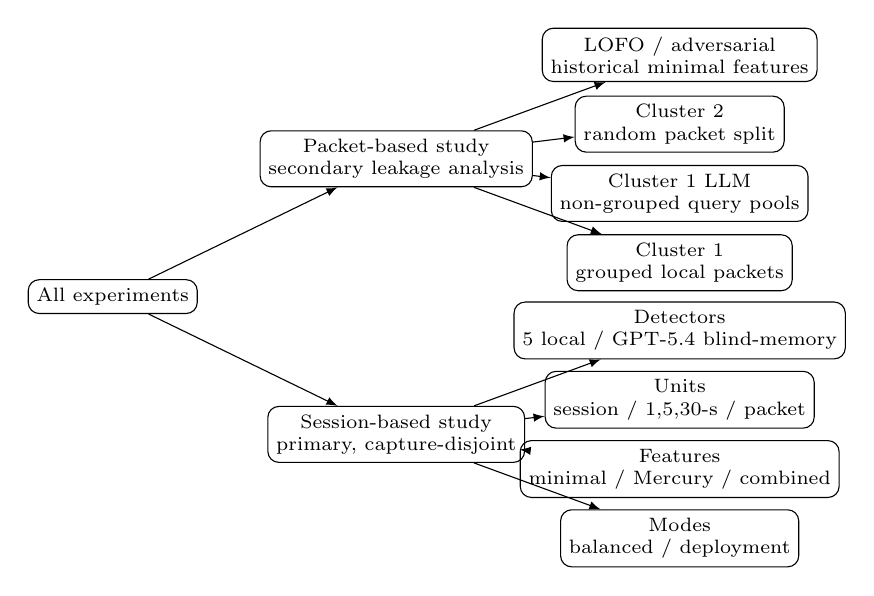
\begin{tikzpicture}[
  grow=right,
  level distance=3.6cm,
  level 1/.style={sibling distance=3.5cm},
  level 2/.style={sibling distance=0.88cm},
  edge from parent/.style={draw,-latex},
  every node/.style={draw,rounded corners,align=center,font=\scriptsize,inner sep=3pt}
]
\node {All experiments}
 child {node {Session-based study\\primary, capture-disjoint}
   child {node {Modes\\balanced / deployment}}
   child {node {Features\\minimal / Mercury / combined}}
   child {node {Units\\session / 1,5,30-s / packet}}
   child {node {Detectors\\5 local / GPT-5.4 blind-memory}}
 }
 child {node {Packet-based study\\secondary leakage analysis}
   child {node {Cluster 1\\grouped local packets}}
   child {node {Cluster 1 LLM\\non-grouped query pools}}
   child {node {Cluster 2\\random packet split}}
   child {node {LOFO / adversarial\\historical minimal features}}
 };
\end{tikzpicture}
\caption{Experiment tree. Dimensions below the session node form a Cartesian product except that GPT-5.4 uses only five-second windows and packet ablation has no memory condition.}
\label{fig:experiment-tree}
\end{figure*}

\begin{table*}[t]
\centering
\caption{Best and worst audited combinations within each primary detector/mode. Values are Accuracy/$F_1^{\mathrm{mal}}$/Recall.}
\label{tab:best-worst}
\footnotesize
\begin{tabularx}{\textwidth}{llX X}
\toprule
Mode & Detector & Best combination & Worst combination \\
\midrule
Balanced & Local & LGBM, minimal, 30-s window: 82.37/84.28/79.50\% & LGBM, Mercury, session: 69.50/60.61/62.21\% \\
Balanced & GPT-5.4 & Blind, minimal, 5-s window: 64.62/66.83/73.85\% & Blind, minimal, packet: 43.85/0.00/0.00\% \\
Deployment & Local & XGB, Mercury, packet: 87.75/82.51/88.98\% & CART, minimal, packet: 65.79/54.80/69.95\% \\
Deployment & GPT-5.4 & Memory, minimal, session: 60.36/57.25/91.59\% & Memory, combined, 5-s window: 46.55/31.24/56.14\% \\
\bottomrule
\end{tabularx}
\end{table*}

\section{Experimental Results}
\label{sec:results}

\subsection{Experiment Matrix}

Table~\ref{tab:experiment-matrix} and Figure~\ref{fig:experiment-tree} define the complete evaluation. The session suite is primary; the older packet study is reported second because its prediction unit and leakage controls differ.

\subsubsection{Technical Summary}
We present here a high-level summary of all results before delving into specificities of different experiments and runs. This allows readers to get an overview of results and best/worst executions without having to go through the entire set of tables and results. In summary:
\begin{itemize}
    \item Across the all test suites, local ML leads every evaluation-mode/prediction-unit comparison. 
    \item Under balanced session/window detection, the strongest model is LGBM on minimal 30-second windows ($F_1=84.28\%$), while GPT-5.4 peaks at $66.83\%$ on blind minimal five-second windows. Under real-world deployment tests where benign traffic significantly outweighs malicious traffic, local LGBM reaches $79.17\%$ session/window $F_1$; GPT-5.4 reaches $57.25\%$ with memory and whole-session minimal features, but obtains its 91.59\% recall with only 55.36\% specificity (see Table~\ref{tab:best-worst}). 
    \item Mercury-style metadata are most useful for deployment packet models, whereas combined features yield the highest mean deployment local $F_1$ across all configurations.
    \item Neither feature expansion improves the LLM enough to justify choosing them over classical ML algorithms and tree ensembles. 
    \item Local prediction takes approximately 0.003~ms/sample versus 1.4--1.9~s per remote call, excluding local feature extraction but including provider/network latency. 
    \item The complementary, packet-only results from the second C1-C2 Experiment set are not contradictory: they answer an easier packet task and, for the LLM query pools and all of Cluster~2, have weaker leakage controls.
\end{itemize}


\subsection{Session-Based Experiments}

\subsubsection{Scope, Sources, and Metric Definitions}
Table~\ref{tab:session-scope} fixes the interpretation boundary. Detection rate is malicious recall; $F_1^{\mathrm{mal}}$ is the harmonic mean of malicious precision and recall; specificity exposes false alarms. ``Balanced'' describes the sampled cohort before whole-capture splitting, not every held-out fold. ``Deployment'' preserves sampled corpus prevalence and uses validation-selected thresholds. Pooled counts below are evaluation appearances across repeated folds, not unique entities.

\begin{table}[h]
\centering
\caption{Held-out LLM test predictions per feature/context variant.}
\label{tab:session-llm-subsets}
\footnotesize
\begin{tabular}{llrrr}
\toprule
Mode & Unit & $N$ & B/M & Mal. \\
\midrule
Balanced & Session/5-s & 106 & 53/53 & 50.00\% \\
Balanced & Packet & 130 & 65/65 & 50.00\% \\
Deployment & Session/5-s & 275 & 184/91 & 33.09\% \\
Deployment & Packet & 275 & 209/66 & 24.00\% \\
\bottomrule
\end{tabular}
\end{table}

\begin{table*}[t]
\centering
\caption{Scope, sources, and metric definitions for the primary session suite.}
\label{tab:session-scope}
\footnotesize
\begin{tabularx}{\textwidth}{p{2.1cm}X}
\toprule
Item & Definition \\
\midrule
Scope & Twelve captures: seven benign and five malware-family captures; capture-disjoint train/validation/test repeated holdout. \\
Sources & Frozen split manifests plus publication artifacts \texttt{session\_local\_results\_\{balanced,deployment\}.json} and \texttt{session\_llm\_results\_\{balanced\_paper\_5k,deployment\_paper\_6k\}.json}. \\
Metrics & Accuracy; malicious precision, recall/detection rate, and $F_1$; specificity; latency; token volume. \\
Uncertainty & Mean $\pm$ sample standard deviation over 10 local or 5 LLM repeats; normal-approximation 95\% intervals are descriptive, not independent-sample guarantees. \\
\bottomrule
\end{tabularx}
\end{table*}


\begin{table}[t]
\centering
\caption{Local cohorts and pooled complete test-fold appearances.}
\label{tab:session-local-cohorts}
\footnotesize
\resizebox{\columnwidth}{!}{%
\begin{tabular}{llrrrr}
\toprule
Mode & Unit & Cohort & Cohort mal. & Test B/M & Test mal. \\
\midrule
Balanced & Session/windows & 6{,}000 & 50.00\% & 8{,}552/17{,}396 & 67.04\% \\
Balanced & Packet ablation & 3{,}000 & 50.00\% & 5{,}663/5{,}688 & 50.11\% \\
Deployment & Session/windows & 6{,}000 & 38.52\% & 13{,}801/9{,}697 & 41.27\% \\
Deployment & Packet ablation & 3{,}000 & 31.57\% & 7{,}561/3{,}752 & 33.17\% \\
\bottomrule
\end{tabular}}
\end{table}

\subsubsection{Local ML Cohorts and Full Held-Out Folds}

The local grid comprises three feature sets, five prediction units, five algorithms, and two prevalence modes. Each of the 150 feature/unit/algorithm/mode summaries contains 10 capture-grouped repeats, for 1{,}500 held-out evaluations. The same frozen cohort and split manifest is reused by every algorithm within a feature/unit/mode cell; model selection therefore does not change the held-out entities. Table~\ref{tab:session-local-grid} reports the best mean malicious $F_1$ within each cell rather than suppressing the less favorable units.

\begin{table*}[t]
\centering
\caption{Best local model per feature set and prediction unit. Values are malicious $F_1$ mean $\pm$ sample standard deviation (percentage points) over 10 capture-grouped repeats. Selection is descriptive across RF, XGB, LGBM, CART, and KNN.}
\label{tab:session-local-grid}
\footnotesize
\resizebox{\textwidth}{!}{%
\begin{tabular}{lllcc}
\toprule
Features & Unit & Balanced model & Balanced $F_1$ & Deployment model and $F_1$ \\
\midrule
\multirow{5}{*}{Minimal}
 & Session & LGBM & $83.89 \pm 18.29$ & LGBM: $76.49 \pm 23.55$ \\
 & 1-s window & LGBM & $84.24 \pm 18.11$ & LGBM: $78.85 \pm 21.60$ \\
 & 5-s window & LGBM & $83.97 \pm 18.04$ & LGBM: $77.71 \pm 22.23$ \\
 & 30-s window & LGBM & $84.28 \pm 18.13$ & LGBM: $79.17 \pm 21.46$ \\
 & Packet & XGB & $75.34 \pm 19.83$ & LGBM: $68.09 \pm 20.85$ \\
\midrule
\multirow{5}{*}{Mercury}
 & Session & CART & $77.89 \pm 24.29$ & XGB: $77.78 \pm 19.98$ \\
 & 1-s window & CART & $72.60 \pm 26.39$ & XGB: $78.54 \pm 19.38$ \\
 & 5-s window & CART & $77.68 \pm 23.94$ & XGB: $78.57 \pm 19.17$ \\
 & 30-s window & CART & $73.91 \pm 24.70$ & LGBM: $78.63 \pm 23.65$ \\
 & Packet & CART & $82.04 \pm 17.28$ & XGB: $82.51 \pm 26.92$ \\
\midrule
\multirow{5}{*}{Combined}
 & Session & LGBM & $77.61 \pm 26.21$ & LGBM: $78.20 \pm 19.30$ \\
 & 1-s window & CART & $79.54 \pm 22.65$ & XGB: $78.89 \pm 19.62$ \\
 & 5-s window & LGBM & $77.61 \pm 26.22$ & XGB: $78.87 \pm 19.67$ \\
 & 30-s window & LGBM & $77.60 \pm 26.22$ & XGB: $78.83 \pm 19.77$ \\
 & Packet & CART & $81.60 \pm 18.79$ & XGB: $82.25 \pm 26.93$ \\
\bottomrule
\end{tabular}}
\end{table*}

Whole-capture grouping produces intentionally heterogeneous folds. Balanced session/window test prevalence spans 0.08--90.27\%, balanced packet prevalence spans 19.48--78.01\%, and the corresponding deployment ranges are 14.52--61.83\% and 5.95--68.30\%. This variation explains the 17--27 point standard deviations in Table~\ref{tab:session-local-grid}; it is also the behavior that a row-random split would conceal. Consequently, differences of a few mean points should not be read as statistically resolved rankings.

\paragraph{Temporal context.}
For minimal features, LGBM is remarkably consistent across the four temporal representations: balanced $F_1$ lies between 83.89\% and 84.28\%, and deployment $F_1$ lies between 76.49\% and 79.17\%. The 30-s window is the best mean result in both modes, but its margin over one-second, five-second, and whole-session variants is smaller than the between-capture variation. Thus, longer context is not monotonically better in this corpus. Mercury and combined representations behave differently: their strongest result is frequently the packet ablation, especially under deployment, where XGB--Mercury reaches $F_1=82.51\%$. This is evidence that richer metadata benefit some local packet decisions, not evidence that packets are the more appropriate operational unit for behavioral attacks.

\subsubsection{Budgeted LLM Test Subsets}

The LLM grid contains 15 feature/unit/context variants per prevalence mode. Whole-session and five-second representations are tested blind and with training-memory context; the packet ablation is blind only. Each row in Table~\ref{tab:session-llm-grid} averages five capture-grouped repeats. Balanced prompting produced 1{,}662 test predictions across all variants at a fixed 0.5 threshold. Deployment consumed 6{,}000 calls: 1{,}875 validation calls and 4{,}125 held-out tests. These are budgeted subsets, whereas local models score complete held-out folds; comparisons therefore concern the same protocol family but not equal test denominators.

\begin{table*}[t]
\centering
\caption{Complete budgeted GPT-5.4 grid. Values are malicious $F_1$ mean $\pm$ sample standard deviation (percentage points) over five repeats. Deployment thresholds are the repeat mean and observed range after validation-only $F_1$ selection on 25 prompts. B denotes blind and M denotes training-memory context.}
\label{tab:session-llm-grid}
\footnotesize
\resizebox{\textwidth}{!}{%
\begin{tabular}{lllrrl}
\toprule
Features & Unit & Context & Balanced $F_1$ & Deployment $F_1$ & Deployment threshold mean [range] \\
\midrule
\multirow{5}{*}{Minimal}
 & Session & B & $10.3 \pm 10.6$ & $49.2 \pm 32.1$ & 0.088 [0.000, 0.140] \\
 & Session & M & $49.2 \pm 38.1$ & $57.3 \pm 32.4$ & 0.070 [0.000, 0.160] \\
 & 5-s window & B & $66.8 \pm 10.8$ & $51.6 \pm 33.4$ & 0.188 [0.000, 0.290] \\
 & 5-s window & M & $52.0 \pm 34.7$ & $54.4 \pm 31.5$ & 0.088 [0.000, 0.200] \\
 & Packet & B & $0.0 \pm 0.0$ & $31.8 \pm 31.0$ & 0.204 [0.130, 0.290] \\
\midrule
\multirow{5}{*}{Mercury}
 & Session & B & $27.6 \pm 17.6$ & $40.3 \pm 35.8$ & 0.068 [0.000, 0.340] \\
 & Session & M & $43.7 \pm 37.3$ & $43.8 \pm 24.4$ & 0.400 [0.000, 0.500] \\
 & 5-s window & B & $14.5 \pm 19.5$ & $45.4 \pm 30.0$ & 0.000 [0.000, 0.000] \\
 & 5-s window & M & $44.1 \pm 36.7$ & $41.1 \pm 22.0$ & 0.672 [0.000, 0.970] \\
 & Packet & B & $47.8 \pm 23.2$ & $48.8 \pm 45.2$ & 0.358 [0.000, 0.500] \\
\midrule
\multirow{5}{*}{Combined}
 & Session & B & $26.8 \pm 21.3$ & $37.7 \pm 30.1$ & 0.054 [0.000, 0.180] \\
 & Session & M & $47.1 \pm 37.8$ & $48.7 \pm 27.5$ & 0.310 [0.000, 0.500] \\
 & 5-s window & B & $35.8 \pm 20.4$ & $45.3 \pm 30.0$ & 0.190 [0.000, 0.950] \\
 & 5-s window & M & $59.9 \pm 22.4$ & $31.2 \pm 26.6$ & 0.586 [0.000, 0.980] \\
 & Packet & B & $56.0 \pm 28.2$ & $50.7 \pm 45.8$ & 0.220 [0.000, 0.290] \\
\bottomrule
\end{tabular}}
\end{table*}

\paragraph{Blind versus training-memory prompts.}
Memory supplies labeled examples and family context from training data only; it does not update model weights. Across the six paired balanced session/window variants, memory raises mean $F_1$ from 30.32\% to 49.34\% and pooled accuracy from 55.82\% to 70.60\%. The gain is not universal: the best balanced row is the blind minimal five-second window at $F_1=66.83\%$, and memory reduces that cell to 51.98\%. Under deployment, memory raises pooled accuracy from 43.94\% to 55.21\%, but mean $F_1$ moves only from 44.93\% to 46.09\%; pooled recall falls from 88.46\% to 56.96\% because the selected operating thresholds differ. These results support training-memory as a useful prompt ablation, not as a substitute for a matched fine-tuned LLM baseline.

\paragraph{Threshold stability.}
The 25 validation prompts per deployment repeat are too few to estimate a stable operating point. Threshold ranges cover zero for 12 of 15 variants and extend to 0.95--0.98 for two combined-window variants. Most starkly, blind Mercury five-second windows select threshold zero in every repeat, producing 100\% malicious recall and 0\% specificity. This is a formally valid optimum under validation $F_1$, but an unusable detector. We therefore interpret deployment recall only alongside precision and specificity and do not claim an operational false-positive rate.

\subsubsection{Headline Detector Comparison}

\begin{table*}[t]
\centering
\caption{Highest-$F_1$ detector within each mode, detector class, and prediction unit.}
\label{tab:session-headline}
\footnotesize
\resizebox{\textwidth}{!}{%
\begin{tabular}{lllllrrrr}
\toprule
Mode & Detector & Unit & Model/context & Features/representation & Acc. & $F_1$ & Prec. & Rec./Spec. \\
\midrule
Balanced & Local & Session/window & LGBM & Minimal, 30-s window & 82.37 & 84.28 & 96.81 & 79.50/82.89 \\
Balanced & Local & Packet & CART & Mercury, packet & 82.31 & 82.04 & 79.43 & 91.59/79.25 \\
Balanced & GPT-5.4 & Session/window & Blind & Minimal, 5-s window & 64.62 & 66.83 & 64.42 & 73.85/55.38 \\
Balanced & GPT-5.4 & Packet & Blind & Combined, packet & 71.54 & 56.01 & 100.00 & 43.08/100.00 \\
Deployment & Local & Session/window & LGBM & Minimal, 30-s window & 85.76 & 79.17 & 86.78 & 82.66/89.70 \\
Deployment & Local & Packet & XGB & Mercury, packet & 87.75 & 82.51 & 84.79 & 88.98/88.98 \\
Deployment & GPT-5.4 & Session/window & Memory & Minimal, session & 60.36 & 57.25 & 53.18 & 91.59/55.36 \\
Deployment & GPT-5.4 & Packet & Blind & Combined, packet & 75.64 & 50.67 & 60.36 & 63.80/80.00 \\
\bottomrule
\end{tabular}}
\end{table*}

Local ML leads all eight matched headline rows by malicious $F_1$. The closest LLM is the balanced blind minimal five-second window, still 17.45 percentage points behind the strongest balanced local session/window detector. The best deployment LLM favors sensitivity, but its precision and specificity remain far below the local operating point.

\begin{figure*}[t]
    \centering
    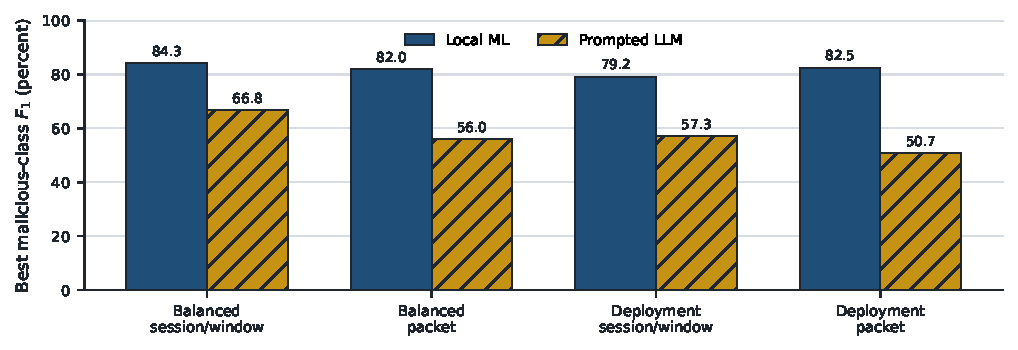
\includegraphics[width=0.92\textwidth]{session_headline_f1.pdf}
    \caption{Highest malicious $F_1$ within each detector-class, prevalence-mode, and prediction-unit comparison. The selected local and prompted-LLM bars need not use the same feature set or context; Table~\ref{tab:session-headline} identifies each winner.}
    \label{fig:session-headline-f1}
\end{figure*}

Figure~\ref{fig:session-headline-f1} makes two gaps visible. First, local models lead prompted LLMs for both temporal and packet units in both prevalence modes. Second, changing from a balanced cohort to corpus-prevalence deployment does not close the gap: the best deployment local packet model reaches 82.51\% $F_1$, whereas the best deployment LLM packet ablation reaches 50.67\%. Because each bar is selected from a different candidate set and the folds are dependent, the figure is a detector-class summary rather than a significance test.

\subsubsection{Feature-Set Comparison}

\begin{table*}[t]
\centering
\caption{Feature-set summary. Local winner mean first selects the best algorithm for each of five units; LLM mean covers five context/unit variants.}
\label{tab:session-features}
\footnotesize
\begin{tabularx}{\textwidth}{llrrXrX}
\toprule
Mode & Features & Mean local $F_1$ & Winner mean & Best local & Mean LLM $F_1$ & Best LLM \\
\midrule
Balanced & Minimal & 75.01 & 82.35 & LGBM, 30-s: 84.28 & 35.67 & Blind 5-s: 66.83 \\
Balanced & Mercury & 69.87 & 76.82 & CART, packet: 82.04 & 35.55 & Blind packet: 47.82 \\
Balanced & Combined & 75.22 & 78.79 & CART, packet: 81.60 & 45.14 & Memory 5-s: 59.93 \\
Deployment & Minimal & 70.42 & 76.06 & LGBM, 30-s: 79.17 & 48.85 & Memory session: 57.25 \\
Deployment & Mercury & 75.34 & 79.21 & XGB, packet: 82.51 & 43.87 & Blind packet: 48.77 \\
Deployment & Combined & 76.23 & 79.41 & XGB, packet: 82.25 & 42.74 & Blind packet: 50.67 \\
\bottomrule
\end{tabularx}
\end{table*}

Minimal features are not merely a weak ablation: they produce the best session/window detectors and the best deployment LLM average. Mercury-style fields are useful for deployment packet models, and the combined set has the strongest mean deployment local result, but the union does not beat the best minimal session model. For GPT-5.4, combined features help on balanced average but hurt deployment average. This non-monotonicity suggests that additional numeric metadata can dilute rather than clarify prompt evidence.

For local models, combined features obtain the highest deployment winner mean (79.41\%), narrowly ahead of Mercury (79.21\%) and above minimal (76.06\%). That aggregate ranking masks the unit-specific result: minimal is strongest for temporal session/window detection, while Mercury is strongest for deployment packets. The corresponding LLM means are lower and non-monotonic. Combined features improve the balanced LLM mean to 45.14\%, but minimal features remain best in deployment at 48.85\%. More fields therefore do not guarantee a better prompted representation.

\subsubsection{Malware-Family Coverage}

\begin{figure*}[t]
    \centering
    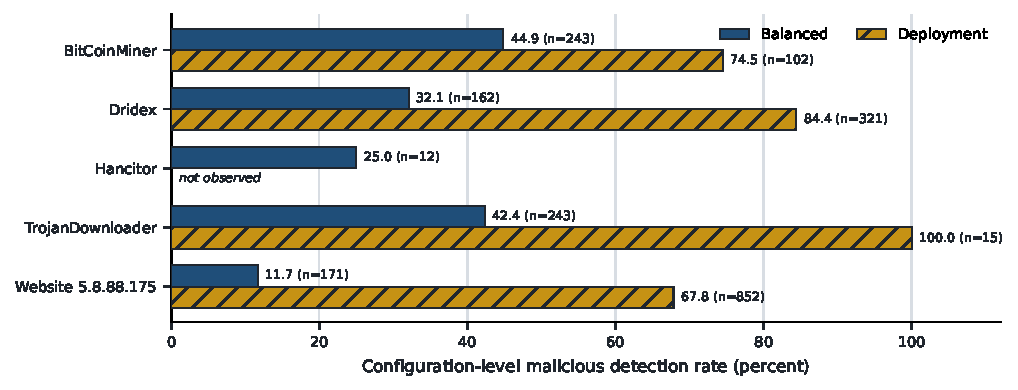
\includegraphics[width=0.92\textwidth]{session_llm_family_detection.pdf}
    \caption{Aggregate GPT-5.4 malicious detection by recorded family over all session-suite feature, context, and unit variants, including packet ablations. Counts are configuration-level prediction rows: the same underlying traffic may recur across variants and is not an independent observation. Hancitor is absent from deployment test subsets.}
    \label{fig:session-family}
\end{figure*}

Figure~\ref{fig:session-family} exposes the limits hidden by aggregate $F_1$. In balanced subsets, detection is 44.86\% for BitCoinMiner (109/243 configuration rows), 32.10\% for Dridex (52/162), 25.00\% for Hancitor (3/12), 42.39\% for TrojanDownloader (103/243), and only 11.70\% for the \texttt{Website\_5.8.88.175} trace (20/171). Deployment rates are 74.51\% for BitCoinMiner (76/102), 84.42\% for Dridex (271/321), 100\% for TrojanDownloader (15/15), and 67.84\% for \texttt{Website\_5.8.88.175} (578/852). The 100\% value has only 15 repeated configuration rows, and Hancitor has no deployment support; neither supports a family-level generalization claim. The local artifacts retain class confusion matrices but not per-family predictions, so a matched local-versus-LLM family comparison cannot be reconstructed and is intentionally omitted.

\subsubsection{Runtime and Deployment Cost}

\begin{table}[t]
\centering
\caption{Median measured prediction latency. Local timing excludes feature extraction; LLM timing includes provider and network delay.}
\label{tab:session-latency}
\footnotesize
\resizebox{\columnwidth}{!}{%
\begin{tabular}{llrrr}
\toprule
Mode & Unit & Local ms & LLM ms & Ratio \\
\midrule
Balanced & Session/window & 0.002912 & 1{,}502.6 & 516{,}041$\times$ \\
Balanced & Packet & 0.002603 & 1{,}490.2 & 572{,}590$\times$ \\
Deployment & Session/window & 0.002897 & 1{,}467.5 & 506{,}517$\times$ \\
Deployment & Packet & 0.002572 & 1{,}437.2 & 558{,}753$\times$ \\
\bottomrule
\end{tabular}}
\end{table}

\begin{figure*}[t]
    \centering
    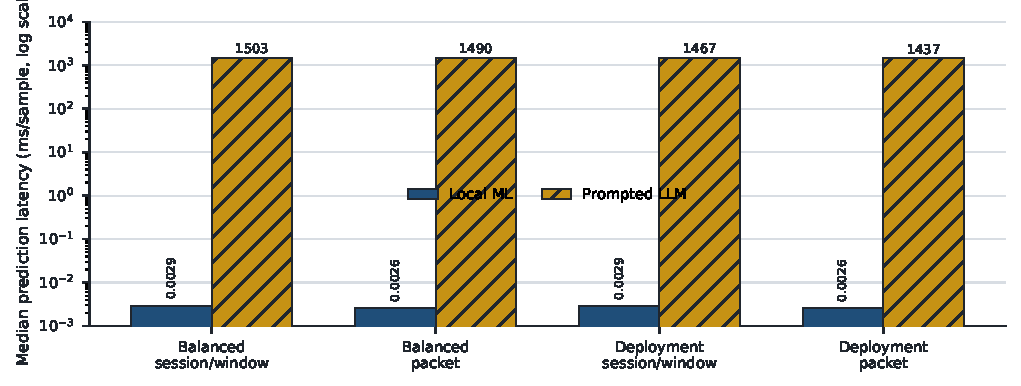
\includegraphics[width=0.92\textwidth]{session_runtime_latency.pdf}
    \caption{Median prediction latency on a logarithmic scale under the timing boundary in Table~\ref{tab:session-latency}. Values are operational measurements, not a hardware-normalized microbenchmark.}
    \label{fig:session-latency}
\end{figure*}

The remote LLM requires 1.44--1.50 seconds per scored sample, compared with approximately 0.0026--0.0029 ms for local prediction. This yields a measured ratio of roughly $0.51$--$0.57$ million to one (Table~\ref{tab:session-latency} and Figure~\ref{fig:session-latency}). The boundary favors local inference because it excludes feature extraction, while the LLM boundary includes network transport and provider queueing. It nonetheless reflects the deployment path actually exercised: a synchronous remote call cannot sustain packet-rate classification without batching, asynchronous concurrency, or local distillation. Token and monetary costs further scale with prompt memory and sequence length, whereas local scoring does not incur a per-decision provider charge.

\subsubsection{Integrity and Inference Limits}

All expected result cells are complete: 15 local configurations by five algorithms by 10 repeats in each prevalence mode, and 15 LLM variants by five repeats in each mode. The archived LLM predictions contain no duplicate result keys or invalid parses, and all 5{,}787 held-out test predictions reconcile with their stored summaries. These checks establish computational completeness, not population validity.

Three limitations constrain inference. First, only 12 capture groups are available, so repeated folds reuse captures and normal-approximation intervals do not represent independent samples. Second, selecting the best row from many algorithms, units, and feature sets introduces winner's optimism; Tables~\ref{tab:session-local-grid}--\ref{tab:session-features} should be read descriptively. Third, the deployment cohorts preserve this corpus's prevalence (38.52\% malicious for session/windows and 31.57\% for packets), not a production network's much lower base rate. Precision and alert burden therefore cannot be extrapolated to enterprise traffic without recalibration. Together with sparse family support and unstable 25-prompt thresholds, the evidence supports comparative claims about this session suite, but not all-family or production-readiness claims.

\subsection{Packet-Based Experiments and Leakage Analysis}

\subsubsection{Cluster 1: Grouped Classical Packets and Non-Grouped LLM Queries}

Cluster~1 is the stronger complementary packet-based protocol. It enforces grouped holdout by session and capture for classical models, repairs malware-family labels for LOFO, and excludes invalid adversarial parses. Its packet-prompt LLM queries and few-shot pools, however, are not explicitly group-disjoint, so they do not inherit the classical split guarantee.

\paragraph{Classical grouped holdout.}
Table~\ref{tab:strict-classical} reports the seven original classical baselines. CART and KNN, together with RF/XGB/LGBM below, remain strongest on mixed and encrypted packets. On E1, CART reaches 98.98\% accuracy ($F_1^{\mathrm{mal}}=0.9827$) under session holdout and 97.68\% ($F_1^{\mathrm{mal}}=0.9624$) under capture holdout; KNN reaches 98.91\% and 97.85\%. The realism penalty is clearest on encrypted capture holdout: accuracy remains above 98\%, but malicious $F_1$ falls to 0.6048 for KNN and 0.4775 for CART. Accuracy alone is therefore misleading under the held-out class skew.

\begin{table*}[t]
\centering
\caption{Cluster~1 classical baselines. Each cell reports Accuracy with malicious-class $F_1$ in parentheses. E1 and E2 are packet-level tasks under group-disjoint holdout. E3 is encrypted-only.}
\label{tab:strict-classical}
\footnotesize
\begin{tabular}{lcccccc}
\toprule
Algorithm & E1 Session & E1 Capture & E2 Session & E2 Capture & E3 Session & E3 Capture \\
\midrule
LR   & 0.7924 (0.5847) & 0.8449 (0.6722) & 0.8084 (0.5642) & 0.8413 (0.6619) & -- & -- \\
LDA  & 0.8216 (0.5997) & 0.8307 (0.6307) & 0.7796 (0.4627) & 0.8293 (0.6248) & -- & -- \\
KNN  & 0.9891 (0.9816) & 0.9785 (0.9655) & 0.9808 (0.9682) & 0.9796 (0.9667) & 0.9946 (0.9137) & 0.9879 (0.6048) \\
CART & 0.9898 (0.9827) & 0.9768 (0.9624) & 0.9848 (0.9748) & 0.9840 (0.9738) & 0.9940 (0.9020) & 0.9845 (0.4775) \\
NB   & 0.7858 (0.4688) & 0.7890 (0.5054) & 0.7549 (0.4205) & 0.7890 (0.5121) & -- & -- \\
SVC  & 0.2490 (0.3529) & 0.2474 (0.3708) & 0.8205 (0.6061) & 0.8375 (0.6684) & -- & -- \\
MLP  & 0.9639 (0.9359) & 0.9698 (0.9506) & 0.9533 (0.9216) & 0.9376 (0.8956) & -- & -- \\
\bottomrule
\end{tabular}
\end{table*}

Table~\ref{tab:strict-llm} summarizes the Cluster~1 runs. On packet-level prompts, GPT-5.4 remains far below classical ML: 50.8\% zero-shot, 68.0\% at the best few-shot setting ($k=10$), and 57.0\% for chain-of-thought. LOFO packet prompting reaches 61.8\% overall. The most interesting result in Cluster~1 is the 4E five-packet window, which reaches 96.0\% accuracy on the smallest tested window and a fixed balanced cohort of 200 sessions, but detection is not stable.

Accuracy drops to 59.5\% at 10 packets and to chance-level behavior at 20 and 50 packets, even while token and latency costs rise substantially. This suggests that the model can exploit some very short-range local structure but does not scale to longer windowed reasoning under the same minimal feature set.

4B uses packet exemplars rather than session windows and each query is evaluated independently, so the increase from 50.8\% zero-shot to 68.0\% at $k=10$ is probably attributed to in-prompt calibration from additional labeled packet exemplars.

\begin{table*}[t]
\centering
\caption{Cluster~1 LLM results. Experiments 4A--4D are packet-level tasks; 4E is session-level on fixed 200-session cohort.}
\label{tab:strict-llm}
\footnotesize
\begin{tabular}{lrrrrrrrr}
\toprule
Experiment & Accuracy & $F_1^{\mathrm{mal}}$ & TP & FP & FN & TN & Tokens & Avg.\ latency \\
\midrule
4A zero-shot   & 0.5080 & 0.2013 & 31  & 27  & 219 & 223 & 194{,}406 & 2.26 s/call \\
4B few-shot $k=1$  & 0.5067 & 0.1957 & 18  & 16  & 132 & 134 & 123{,}877 & 1.78 s/call \\
4B few-shot $k=3$  & 0.5400 & 0.4103 & 48  & 36  & 102 & 114 & 153{,}266 & 2.09 s/call \\
4B few-shot $k=5$  & 0.6100 & 0.5412 & 69  & 36  & 81  & 114 & 181{,}411 & 2.19 s/call \\
4B few-shot $k=10$ & 0.6800 & 0.5932 & 70  & 16  & 80  & 134 & 254{,}648 & 2.05 s/call \\
4C chain-of-thought & 0.5700 & 0.5376 & 50  & 36  & 50  & 64  & 165{,}933 & 6.85 s/call \\
4D LOFO overall  & 0.6180 & 0.5979 & 142 & 83  & 108 & 167 & 364{,}172 & -- \\
4E session $w=5$  & 0.9600 & 0.9615 & 100 & 8   & 0   & 92  & 134{,}582 & 2.51 s/call \\
4E session $w=10$ & 0.5950 & 0.7117 & 100 & 81  & 0   & 19  & 184{,}903 & 2.88 s/call \\
4E session $w=20$ & 0.5050 & 0.6689 & 100 & 99  & 0   & 1   & 281{,}833 & 3.08 s/call \\
4E session $w=50$ & 0.5000 & 0.6667 & 100 & 100 & 0   & 0   & 570{,}808 & 4.22 s/call \\
\bottomrule
\end{tabular}
\end{table*}

\paragraph{Family generalization.}
Table~\ref{tab:strict-lofo} and Figure~\ref{fig:lofo-family} show the repaired-family LOFO analysis. The session-holdout classical baselines remain strong: best-family accuracy ranges from 85.21\% (HTTPS Trojan) to 98.62\% (BitCoinMiner). Capture-holdout LOFO is more demanding, with best-family accuracy ranging from 67.48\% (Hancitor) to 75.80\% (TrojanDownloader). Cluster~1 LLMs never exceed the best session-holdout classical result and ranges from 49.0\% (TrojanDownloader) to 79.0\% (BitCoinMiner). The largest gaps appear on Dridex and TrojanDownloader, where the LLM remains far below the best classical model despite having access to few-shot examples from the other families.

\begin{table*}[t]
\centering
\caption{Cluster~1 LOFO results by held-out family. Classical columns report the best model for that family and split; values are Accuracy/$F_1^{\mathrm{mal}}$.}
\label{tab:strict-lofo}
\footnotesize
\begin{tabular}{lccc}
\toprule
Held-out family & Best session classical & Best capture classical & LLM \\
\midrule
BitCoinMiner & CART 0.9862/0.9862 & CART 0.7569/0.8029 & 0.790/0.800 \\
Dridex & KNN 0.9283/0.9241 & CART 0.7579/0.8043 & 0.550/0.563 \\
Hancitor & CART 0.9042/0.8955 & CART 0.6748/0.7167 & 0.610/0.465 \\
TrojanDownloader & CART 0.9836/0.9835 & CART 0.7580/0.8038 & 0.490/0.571 \\
HTTPS Trojan & KNN 0.8521/0.8284 & CART 0.7162/0.7569 & 0.650/0.533 \\
\bottomrule
\end{tabular}
\end{table*}

\begin{figure}[t]
\centering
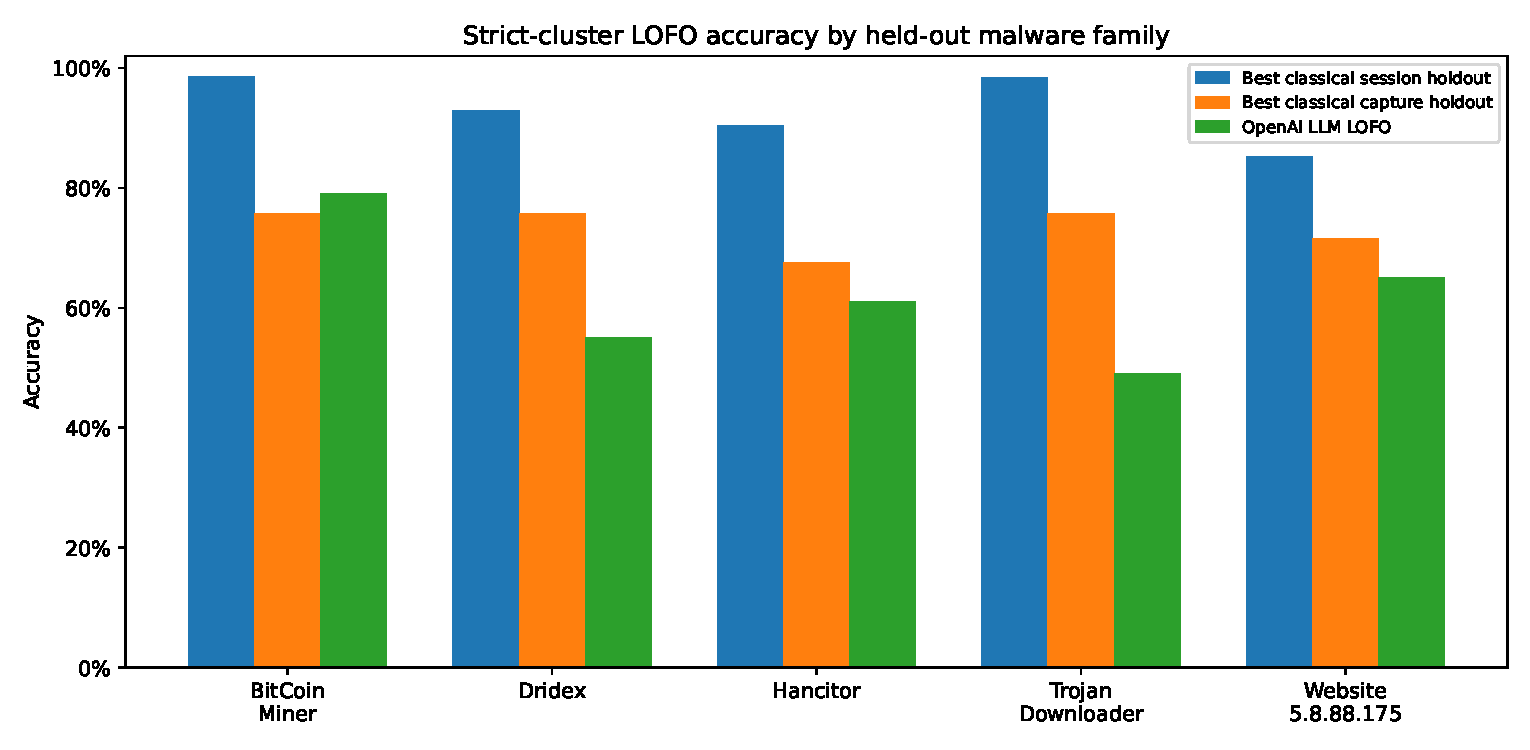
\includegraphics[width=\columnwidth]{lofo_family_comparison.pdf}
\caption{Cluster~1 LOFO accuracy by held-out family. The best session-holdout classical model remains above LLMs for every family.}
\label{fig:lofo-family}
\end{figure}

\paragraph{Adversarial robustness.}

The adversarial experiments are easier to be read as four separate questions. 
\begin{itemize}
    \item Packet-level evasion asks whether a perturbed malicious packet is relabeled as normal. 
    \item Transfer asks whether a perturbation designed against one model also fools another model without any further modification. Transfer is included because the LLM is treated as a black-box API and does not expose gradients or internal scores for direct white-box optimization. We thus first craft adversarial packets against accessible source models on the same five-feature space, specifically CART and KNN, and then submit those unchanged perturbed feature vectors to the LLM.
    \item Session-level consistency asks whether many individually perturbed packets can overturn the majority verdict of a malicious session.
    \item Black-box search and adaptive query complexity ask whether the LLM can be fooled when the attacker only sees model outputs and must search by repeated API queries.
\end{itemize}

The adversarial section is intended as a representation-space robustness study, because both the classical and LLM detectors consume the same engineered side-channel features. The experiment asks whether bounded, physically plausible changes in the deployed feature representation are enough to change decisions. It does not claim that every successful perturbation is a fully replayable end-to-end packet manipulation under arbitrary application semantics. That position is already compatible with current limitations. Also, the study is a purely isolated-point analysis. The Cluster~1 includes session-level perturbation over 200 perturbed sessions, transfer attacks, black-box search, and adaptive query-complexity analysis. We are careful about distinguishing packet sensitivity from session-level persistence. In that strict setting, packet-level LLM evasion is high, transfer reaches $60–82\%$, and black-box hill-climbing succeeds in $66–82\%$ of cases, but session-level majority detection on perturbed sessions remains $98–99\%$ for the LLM and $91–99\%$ for CART. 

\begin{figure*}[t]
\centering
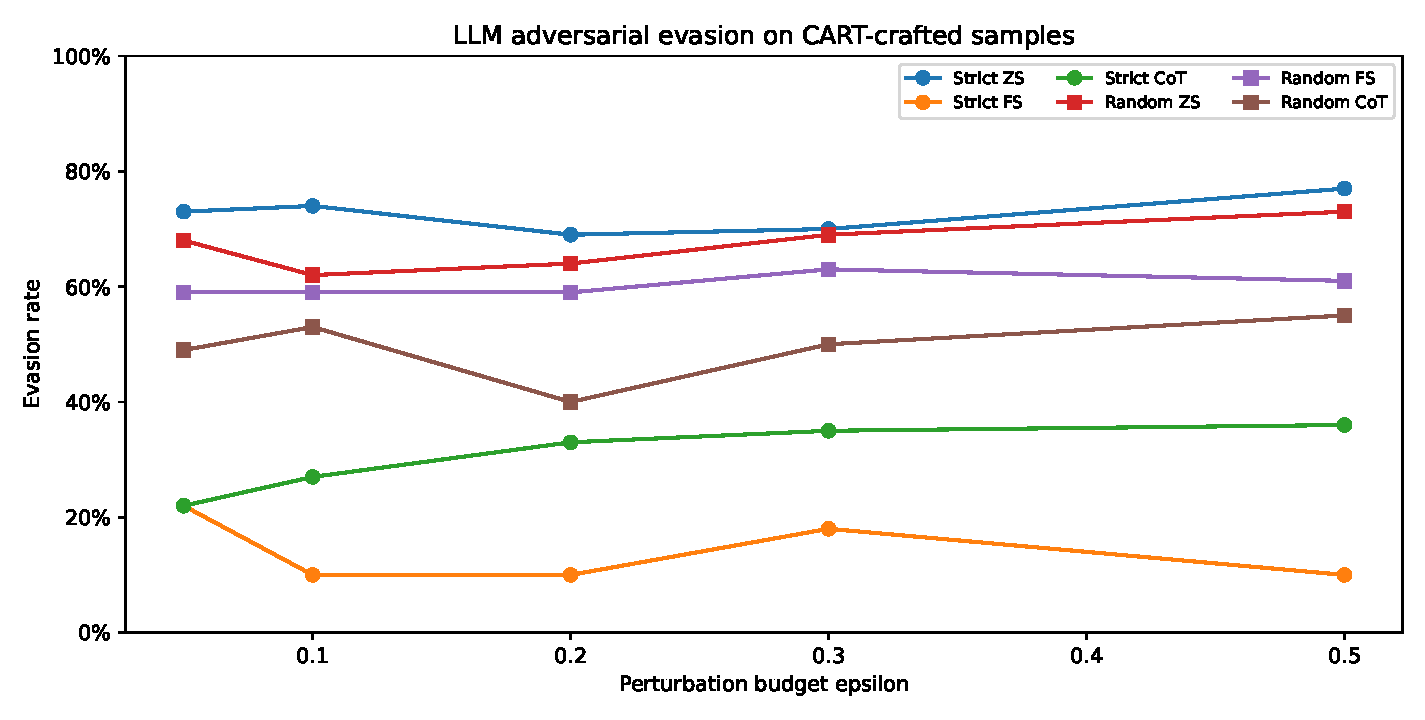
\includegraphics[width=\linewidth]{adversarial_llm_evasion.pdf}
\caption{LLM evasion on CART-crafted adversarial samples. Zero-shot (ZS) vulnerability is high in both clusters; few-shot prompting helps in Cluster~1 but does not close the gap.}
\label{fig:adv-packet-compare}
\end{figure*}

Adversarial evaluation in Cluster~1 covers packet-level evasion, transfer, session-level consistency, black-box search, and adaptive query complexity. Tables~\ref{tab:strict-adv} and ~\ref{tab:strict-tree-ensembles} reports the main packet-level and transfer trends for CART-crafted adversarial samples. Session detection is measured on 100 perturbed sessions; black-box HC denotes hill-climbing evasion against LLMs. CART and KNN packet-level evasion remain in the single digits or low teens, while LLM zero-shot evasion stays between 69\% and 77\%. Few-shot prompting substantially improves LLM robustness on these crafted samples, but evasion still reaches 18\% at $\epsilon=0.30$. Chain-of-thought sits between zero-shot and few-shot. Transfer from CART-crafted samples to the LLM ranges from 60\% to 82\%. On perturbed sessions, however, majority voting remains strong: the LLM session detector stays at 98--99\% across all $\epsilon$ values, slightly above CART at higher budgets. The black-box results are more pessimistic: hill climbing succeeds 66--82\% of the time and random search 84--98\%. Finally, adaptive query-complexity experiments show 95--100\% LLM evasion within a mean of 5.05--7.10 queries and a cost of roughly \$0.015--\$0.021 per successful evasion. Figure \ref{fig:adv-packet-compare} graphically presents these findings showing a clear disadvantage of LLMs against classical algorithms.

\begin{table*}[t]
\centering
\caption{Cluster~1 adversarial summary for CART-crafted samples.}
\label{tab:strict-adv}
\footnotesize
\begin{adjustbox}{width=\textwidth}
\begin{tabular}{ccccccccc}
\toprule
$\epsilon$ & CART evade & KNN evade & LLM ZS evade & LLM FS evade & LLM CoT evade & CART$\rightarrow$LLM transfer & LLM session det. & Black-box HC \\
\midrule
0.05 & 4\%  & 2\% & 73\% & 22\% & 22\% & 62\% & 99\% & 74\% \\
0.10 & 7\%  & 1\% & 74\% & 10\% & 27\% & 60\% & 99\% & 66\% \\
0.20 & 12\% & 4\% & 69\% & 10\% & 33\% & 70\% & 99\% & 82\% \\
0.30 & 9\%  & 1\% & 70\% & 18\% & 35\% & 72\% & 99\% & 82\% \\
0.50 & 9\%  & 1\% & 77\% & 10\% & 36\% & 82\% & 98\% & 78\% \\
\bottomrule
\end{tabular}
\end{adjustbox}
\end{table*}


\paragraph{Tree-ensemble models under Cluster~1 holdout.}
\label{subsec:strict-ensembles}

Cluster~1 also evaluates RF, XGB, and LGBM on the same minimal five-feature representation. Experiments~E1--E3 remain packet-level prediction tasks with train/test separation enforced at the session or capture level. These ensemble runs use independently redrawn packet subsets, so small differences from CART/KNN are corroborative rather than paired wins.

\begin{table*}[t]
\centering
\caption{Cluster~1 tree-ensemble results. Cell reports accuracy with malicious-class $F_1$ in parentheses. E1 and E2 are mixed-traffic packet tasks under grouped holdout, E3 is encrypted-only, and LOFO columns report macro-averages over five held-out malware families.}
\label{tab:strict-tree-ensembles}
\footnotesize
\resizebox{\textwidth}{!}{%
\begin{tabular}{lcccccccc}
\toprule
Algorithm & E1 Session & E1 Capture & E2 Session & E2 Capture & E3 Session & E3 Capture & LOFO Session Avg. & LOFO Capture Avg. \\
\midrule
RF   & 0.9894 (0.9817) & 0.9764 (0.9625) & 0.9878 (0.9794) & 0.7186 (0.6900) & 0.9944 (0.9070) & 0.9954 (0.8194) & 0.8929 (0.8706) & 0.7195 (0.7665) \\
XGB  & 0.9857 (0.9751) & 0.9695 (0.9508) & 0.9866 (0.9774) & 0.7075 (0.6815) & 0.9930 (0.8829) & 0.9886 (0.4237) & 0.9152 (0.9040) & 0.7260 (0.7770) \\
LGBM & 0.9880 (0.9791) & 0.9706 (0.9527) & 0.9864 (0.9771) & 0.7035 (0.6787) & 0.9939 (0.8979) & 0.9881 (0.4073) & 0.9094 (0.8955) & 0.7095 (0.7607) \\
\bottomrule
\end{tabular}%
}
\end{table*}

Table~\ref{tab:strict-tree-ensembles} shows that RF is the strongest of the newly added ensembles on all six grouped-holdout E1--E3 tasks. On mixed session holdout (E1), RF reaches 98.94\% accuracy with malicious-class $F_1=0.9817$, essentially matching the previously reported CART and KNN results (98.98\% / 0.9827 and 98.91\% / 0.9816, respectively). On the limited 20K session-holdout experiment (E2), all three ensemble methods remain near-saturated, with RF again leading at 98.78\%, followed by XGB at 98.66\% and LGBM at 98.64\%. Because this phase was independently resampled, these small advantages over the earlier CART/KNN session-holdout numbers should be read as corroborating competitiveness rather than as definitive paired wins. On encrypted session holdout (E3), RF again remains very close to the best earlier baselines, but KNN still retains a slight edge (99.46\% accuracy and $F_1=0.9137$ versus 99.44\% and $F_1=0.9070$ for RF).

Capture holdout is more discriminative and reveals a less uniform picture. On E1 mixed capture holdout, RF (97.64\%, $F_1=0.9625$) is effectively tied with CART (97.68\%, $F_1=0.9624$) and only marginally below KNN (97.85\%, $F_1=0.9655$), whereas XGB and LGBM are marginally weaker. The strongest negative result appears in E2 limited capture holdout: RF/XGB/LGBM fall to 71.86\%, 70.75\%, and 70.35\% accuracy, with malicious recall near 0.99 but precision only about 0.53, 0.52, and 0.52, respectively. By contrast, the earlier CART and KNN baselines remain near 98\% on the same experimental template. This indicates that the larger ensemble models can become miscalibrated under low-data, capture-shifted training, aggressively over-predicting the malicious class. Encrypted capture holdout (E3) shows the opposite pattern. Here RF is the winner among the newly added ensembles and also surpasses the earlier CART/KNN baselines, reaching 99.54\% accuracy with malicious-class $F_1=0.8194$, compared with 98.79\% / 0.6048 for KNN and 98.45\% / 0.4775 for CART. XGB and LGBM maintain high overall accuracy in this setting, but their malicious recall collapses to roughly 0.30 and 0.29, yielding much weaker malicious-class $F_1$ values of 0.4237 and 0.4073. This is an important reminder that overall accuracy alone is misleading on highly imbalanced encrypted capture holdout.

The LOFO experiments likewise yield a mixed outcome. Averaged over the five held-out malware families, XGB achieves the best ensemble score under session-group LOFO (91.52\% accuracy, $F_1=0.9040$), slightly above the earlier CART average (91.02\%) but still below KNN (92.78\%). LGBM remains close to CART on average (90.94\%), while RF is pulled down by weaker transfer on Dridex (89.29\% average). Family-wise, the best session-LOFO result across all tested classical models is split across learners rather than monopolized by any one method: LGBM is strongest on BitCoinMiner, RF on Hancitor, KNN on Dridex and Website\_5.8.88.175, and CART on TrojanDownloader. Under the stricter capture-group LOFO, XGB obtains the best ensemble average (72.60\%), but CART still remains the strongest overall model on average (73.28\%) and on four of the five held-out families; the only family for which an ensemble clearly leads is Hancitor, where XGB reaches 73.71\%.



\subsubsection{Cluster 2: Random Packet Splits with Session Leakage}

Cluster~2 is used because it captures a more permissive evaluation style that is still common and more generic. Random packet-level train/test partitioning, no repaired-family LOFO, and an LLM evaluated on a pre-fix database provides insights on whether session-specific data can augment or inhibit detection over minimal characteristics. 

Table~\ref{tab:random-classical} shows that the random packet split does not materially change the headline performance of the strongest classical models on the mixed tasks. KNN and CART again operate at approximately 99\% accuracy on E1 and E2, and above 99.5\% on encrypted traffic. This is an important nuance: for the strongest classical methods the biggest realism penalty does not come from session leakage alone, but from harder settings such as capture holdout and family holdout.

\begin{table*}[t]
\centering

\begin{minipage}[t]{0.60\textwidth}
\centering
\captionof{table}{Cluster~2 classical baselines under random packet-level splitting. Each cell reports accuracy with malicious-class $F_1$ in parentheses.}
\label{tab:random-classical}
\footnotesize
\resizebox{\linewidth}{!}{%
\begin{tabular}{lccc}
\toprule
Algorithm & E1 Random & E2 Random & E3 Encrypted Random \\
\midrule
LR   & 0.7866 (0.5676) & 0.8232 (0.6143) & -- \\
LDA  & 0.8066 (0.5548) & 0.8082 (0.5652) & -- \\
KNN  & 0.9913 (0.9856) & 0.9838 (0.9735) & 0.9958 (0.9369) \\
CART & 0.9901 (0.9834) & 0.9863 (0.9774) & 0.9951 (0.9252) \\
NB   & 0.7026 (0.1100) & 0.6960 (0.1041) & -- \\
SVC  & 0.3015 (0.4608) & 0.8195 (0.6155) & -- \\
MLP  & 0.9630 (0.9374) & 0.9508 (0.9162) & -- \\
\bottomrule
\end{tabular}%
}
\end{minipage}
\hfill
\begin{minipage}[t]{0.37\textwidth}
\centering
\captionof{table}{Cluster~2 LLM results. Tokens are total usage per experiment.}
\label{tab:random-llm}
\footnotesize
\resizebox{\linewidth}{!}{%
\begin{tabular}{lccc}
\toprule
Experiment & Accuracy & $F_1^{\mathrm{mal}}$ & Tokens \\
\midrule
4A zero-shot & 0.6240 & 0.4535 & 207{,}992 \\
4B few-shot $k=1$  & 0.6600 & 0.4848 & 141{,}570 \\
4B few-shot $k=3$  & 0.7000 & 0.5909 & 174{,}053 \\
4B few-shot $k=5$  & 0.5900 & 0.5914 & 209{,}861 \\
4B few-shot $k=10$ & 0.6833 & 0.5455 & 325{,}616 \\
4C chain-of-thought & 0.6450 & 0.5235 & 186{,}532 \\
4E session $w=5$  & 0.6000 & 0.3750 & 167{,}631 \\
4E session $w=10$ & 0.5750 & 0.3089 & 229{,}365 \\
4E session $w=20$ & 0.6300 & 0.4861 & 362{,}098 \\
4E session $w=50$ & 0.5477 & 0.6786 & 738{,}988 \\
\bottomrule
\end{tabular}%
}
\end{minipage}

\end{table*}

\paragraph{Cluster~2 packet prompts and session windows.}
The Cluster~2 experimentation produces somewhat higher packet-level LLM scores than the stricter Cluster~1 run: 62.4\% zero-shot, 70.0\% best few-shot (at $k=3$), and 64.5\% CoT. Those gains do not close the gap to classical ML. The session-window story is again unstable. Accuracy ranges from 57.5\% to 63.0\% for 5--20 bi-directional windows and then drops to 54.8\% at 50 packets. Unlike in Cluster~1, experiment 4E does not record per-call latency, and the cohort is not fixed across window sizes, so the 4E numbers are descriptive rather than controlled.

The adversarial archive still shows high LLM susceptibility on minimal features. For CART-crafted samples, LLM zero-shot evasion stays between 62\% and 73\%, few-shot between 59\% and 63\%, and CoT between 40\% and 55\%. Session-level LLM detection on perturbed sessions remains high (96--99\% for $\epsilon \leq 0.30$ in the saved archive). 

\subsubsection{Packet-Based Cluster Comparison}

\begin{table*}[t]
\centering
\caption{High-level comparison between experiment Clusters~1 and ~2.}
\label{tab:cluster-compare}
\footnotesize
\begin{tabularx}{\textwidth}{p{3.2cm}p{3.0cm}p{3.0cm}X}
\toprule
Metric & Cluster~1 strict & Cluster~2 random-leakage & Interpretation \\
\midrule
Split design & Session-group and capture-group holdout & Random 70/30 packet split & Only Cluster~1 supports claims about unseen sessions and unseen captures. \\
LLM provider & OpenAI GPT-5.4 & {OpenAI GPT-5.4 and Claude Sonnet~4.6} & Cross-cluster differences are confounded by methodology. \\
Packet records & 4{,}656{,}613 & 4{,}692{,}639 & The strict cluster uses revised sessionization and a slightly different packet accounting. \\
Best classical E1 accuracy & 98.98\% (CART session) / 97.85\% (KNN capture) & 99.13\% (KNN) & Leakage has limited effect on the easiest classical mixed-packet task; capture holdout is more informative. \\
Best LLM packet accuracy & 68.0\% (4B $k=10$) & 70.0\% (4B $k=3$) & Both remain far below classical ML. \\
Best LLM session-window accuracy & 96.0\% ($w=5$), then 59.5\%, 50.5\%, 50.0\% & 63.0\% ($w=20$) & Session prompting is unstable and non-monotonic in both clusters. \\
LOFO availability & Yes; overall 61.8\% and best classical session-holdout 82.97--98.62\% & No Cluster~2 LOFO & Family claims come from Cluster~1 only. \\
LLM adversarial vulnerability & ZS 69--77\%, transfer 60--82\%, black-box HC 66--82\% & ZS 62--73\%, deprecated transfer JSON & Both clusters indicate vulnerability; only Cluster~1 supports adversarial conclusions. \\
\bottomrule
\end{tabularx}
\end{table*}

Figures~\ref{fig:adv-packet-compare}, \ref{fig:llm-packet-compare},\ref{fig:llm-session-compare} and Table~\ref{tab:cluster-compare} summarize the relationship between the two clusters. Four comparisons are especially important.

First, the classical picture is stable at the top end. KNN and CART are already so strong on the mixed packet tasks that moving from a random packet split to session-group holdout changes little. The more meaningful realism penalties appear when we hold out entire captures and entire malware families, not merely when we prevent within-session leakage.

Second, the LLM story is more sensitive. Cluster~2 reports higher packet-level LLM scores than Cluster~1, but that difference is affected by split design. Thus, we avoid direct attribution. What is clear in both clusters is that the LLM never approaches the strongest classical baselines on the packet tasks.

Third, session-level prompting is brittle rather than uniformly useless. Cluster~1 run achieves an unusually strong 96.0\% at five packets, but the gain does not survive longer bi-directional windows. Cluster~2 run never produces a comparable peak and is likewise unstable across window sizes. Both clusters reject the simple claim that ``more session context monotonically helps'' on this feature representation.

Fourth, adversarial vulnerability is a shared property. Both clusters show high LLM evasion under minimal-feature perturbations. Cluster~1 supports the stronger claim, because it takes into consideration sessions-per-packet and allows for black-box and query-complexity experiments, but Cluster~2 reports point in the same direction.

\section{Discussion}
\label{sec:discussion}

The session suite supports a clear message. Given identical payload-free metadata and capture-disjoint evaluation, supervised local models are more accurate, more stable, and orders of magnitude faster than a general-purpose prompted LLM, even if the LLM is exposed to prior information on similar malicious traffic. The fact that LLM receives temporal context (whole-session or five-second ordered summaries), and memory prompts receive labeled training-only context doesnt seem to alter results in either cluster of experiments, nor is the result different when confined to the deliberately minimal feature set. Mercury-style and combined metadata alter individual winners but do not create a consistent LLM advantage.

Feature expansion has different effects by detector and operating mode. Minimal statistics remain strongest for session/window detection; Mercury-style ports, direction, and service hints improve selected deployment packet models; combined features produce the best mean deployment local score. The LLM is non-monotonic: combined features improve its balanced mean but reduce its deployment mean. A plausible interpretation is representational mismatch: adding numeric fields increases prompt complexity without providing the protocol tokens or payload semantics that language models exploit in richer traffic systems. This interpretation is consistent with, but not proved by, our results.

Balanced and deployment results also answer different questions. Balanced cohorts isolate discrimination under equal sampled class mass. Deployment cohorts expose precision/specificity under this corpus's prevalence and force threshold selection onto validation data. The latter reveals threshold instability rather than production readiness. The legacy random-leakage cluster remains useful only as an optimistic contrast; its higher packet scores cannot establish unseen-session or unseen-capture performance.

\subsection{Context and Memory}

The best balanced GPT-5.4 result uses a blind minimal five-second window, while the best deployment result uses a memory-enabled whole session. Memory improves mean balanced session/window $F_1$ but is not uniformly beneficial and materially changes validation-selected thresholds. Thus, ``more context'' has at least three meanings---longer observed behavior, more metadata fields, and labeled in-prompt memory---and none improves performance monotonically. The historical 4E peak at five packets, followed by collapse at longer windows, is consistent with this new result but is not directly comparable because its cohort and model generation differ.

\subsection{Penalties, LOFO, and adversarial testing}

The old packet results clarify where evaluation matters most. For the strongest classical baselines, preventing within-session packet leakage changes little on easy mixed-packet tasks; holding out complete captures and families is more discriminative. The new session folds make that capture dependence visible through wide prevalence and performance variation. The legacy adversarial evaluation remains representation-space evidence: it shows that bounded feature perturbations can flip LLM outputs, but it does not establish end-to-end packet replayability.

Training-memory and legacy few-shot prompting both sometimes help, but they should not be conflated with supervised fitting. The former is leakage-controlled in-context conditioning; the latter uses a weaker packet pool. Neither matches the amount of labeled optimization received by local models, and no completed fine-tuned LLM result is available for a supervised-to-supervised comparison.

\section{Limitations}
\label{sec:limitations}

The corpus contains only 12 capture groups, with one malicious family per malicious capture. Capture holdout prevents direct capture leakage but cannot disentangle family, environment, and capture effects. It also creates highly heterogeneous folds; balanced session-fold prevalence ranges from 0.08\% to 90.27\%. Deployment prevalence is faithful only to this sampled corpus, not to a production network, where lower malicious prevalence would reduce precision at fixed sensitivity/specificity.

\begin{figure}[t]
\centering
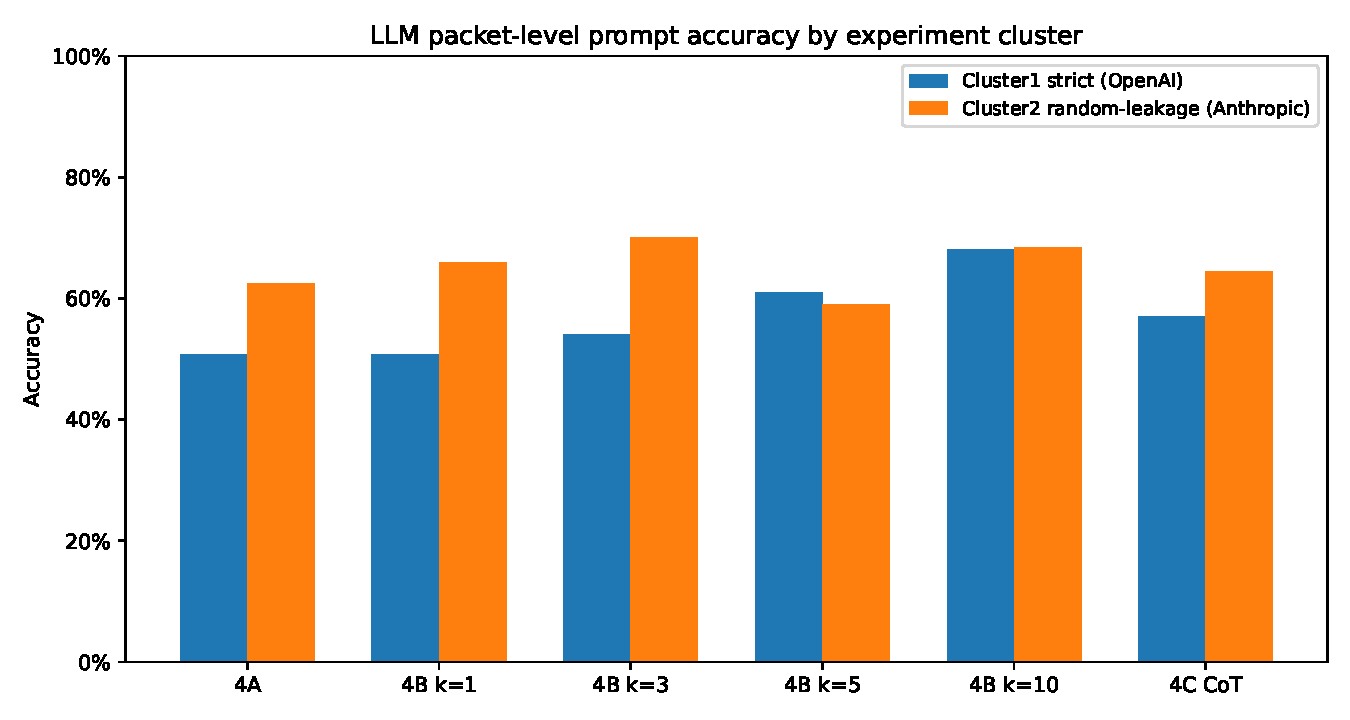
\includegraphics[width=\linewidth]{llm_packet_comparison.pdf}
\caption{Packet-level LLM prompt accuracy by cluster. Cluster~2 yields somewhat higher packet-level scores, but both clusters remain well below classical ML.}
\label{fig:llm-packet-compare}
\end{figure}\hfill
\begin{figure}[t]
\centering
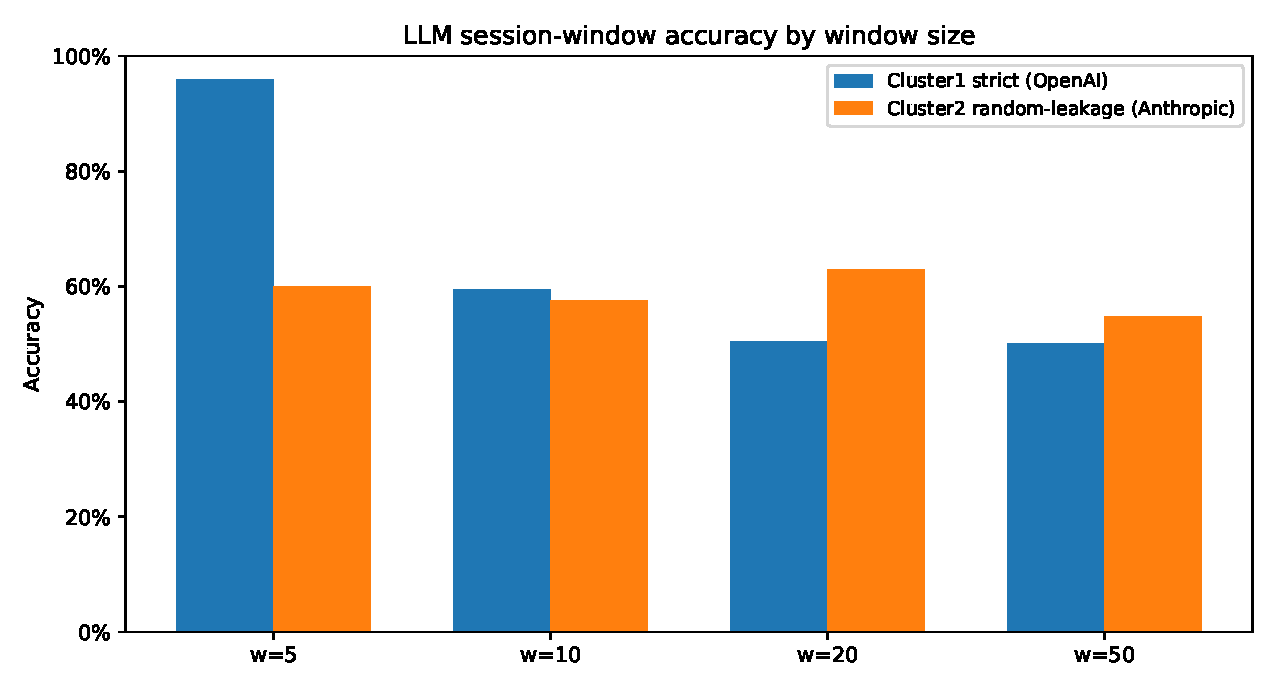
\includegraphics[width=\linewidth]{llm_session_windows.pdf}
\caption{Session-window accuracy by cluster. Cluster~1 peaks at five packets and then collapses, while Cluster~2 remains unstable across all window sizes.}
\label{fig:llm-session-compare}
\end{figure}





The primary LLM evaluation is budgeted: five selected repeats and small held-out subsets rather than ten complete folds. Worst-case binomial uncertainty is already broad, and clustering/reuse makes it larger. Hancitor is absent from deployment LLM tests, TrojanDownloader support is negligible, and 25 validation prompts per repeat are inadequate for a stable operational threshold. Best-row selection across 30 variants further introduces selection optimism. We therefore support comparative and ablation claims, not precise all-family or production detection rates.

Runtime is not hardware normalized. Local timing excludes parsing/feature construction and measures batch prediction; LLM timing includes remote service/network latency. The magnitude supports an operational distinction but not a microarchitectural benchmark. Likewise, Mercury-style features are the 20 fields available in our schema, not Cisco Mercury's full fingerprint implementation.

The session LLM is identified as GPT-5.4 in both the manuscript and archived JSON rows. Provider-side request metadata should nevertheless be retained with the camera-ready artifact so that the served model alias and date can be independently verified. The artifact includes a fine-tuning export/evaluation path, but the audited result set contains no completed matched fine-tuned baseline. Finally, legacy and session generations differ in model, split, sessionization, and sampling; cross-generation comparisons are descriptive rather than causal.


\section{Conclusion}
\label{sec:conclusion}

We evaluated payload-free traffic detection across minimal, Mercury-style, and combined metadata using whole sessions, behavior windows, and packet ablations. Under frozen capture-disjoint repeated holdout, local supervised models lead GPT-5.4 in every matched headline comparison and are approximately half a million times faster under the measured inference boundary. The best balanced session/window $F_1$ is 84.28\% for local LGBM versus 66.83\% for GPT-5.4; under corpus prevalence, the corresponding best values are 79.17\% and 57.25\%. More metadata and training-memory context help selected cases but not monotonically.

The legacy packet experiments explain why protocol discipline matters: grouped classical packet tasks can remain near saturation, while non-grouped prompt pools and random packet splits produce optimistic evidence. The combined results do not show that LLMs are incapable of extracting traffic signal; they show that, on this corpus and payload-free representation, a generic remote LLM is better positioned as asynchronous triage than as a replacement for a fast local detector. Stronger deployment claims require more independent captures, stable low-false-positive thresholding, complete family support, and a matched fine-tuned LLM baseline.

% \section*{Open Science}
% Artifacts and output JSON for all experiments can be found on the project's repository at:
% \href{https://anonymous.4open.science/r/limits-side_channel_features_intrusion_detection-BF3F/README.md}{[ANONYMIZED LINK]}

\bibliographystyle{plain}
\bibliography{references}

\section*{Appendix}
\label{appendix}

We provide artifacts to evaluate (i) payload-free minimal, Mercury-style, and combined features; (ii) capture-disjoint session/window detection under balanced and real-world deployment evaluation; (iii) blind versus training-memory LLM prompting; and (iv) the legacy packet, LOFO, and feature-space adversarial results. We provide an anonymous artifact repository for double-blind review:

The repository is accessible through the direct README link [ANONYMIZED FOR SUBMISSION]:
\begin{center}
\url{https://anonymous.4open.science/r/limits-side_channel_features_intrusion_detection-BF3F/README.md}
\end{center}

No username, password, or private credential is required to inspect the repository during review. Reviewers who wish to rerun API-dependent LLM experiments must supply their own API credentials, as described below. All source code, configuration, split definitions, and available result logs are included anonymously.

\paragraph{Artifact inventory.}
The artifacts needed to evaluate the paper are enumerated below.

\begin{enumerate}
    \item \textbf{Documentation.}
    The repository includes a top-level \texttt{README.md} describing the research objective, experiment phases, latest result summaries, and the major implementation changes in the current artifact version. The dependency list is provided in requirements.txt.

    \item \textbf{Experiment orchestration scripts.}
    The top-level script run\_all.py orchestrates the full pipeline. It exposes separate phases for dataset acquisition, feature extraction, local tree-ensemble baselines, classical ML baselines, LLM experiments, analysis/report generation, and adversarial robustness experiments. The script also provides dry-run and compact-prompt modes, allowing reviewers to inspect prompts and execution paths without issuing paid LLM API calls.

    \item \textbf{Configuration files.}
    The directory configs/ contains config.py, which defines the three feature sets, grouped-holdout parameters, 6{,}000-session and 3{,}000-packet cohorts, LLM budget profiles, memory limits, malware-family registry, adversarial budgets, sessionization, and provider settings.

    \item \textbf{Dataset acquisition and preprocessing code.}
    The file src/download\_datasets.py implements public-capture acquisition, src/feature\_extraction.py extracts packet/session fields, and src/database.py defines the SQLite schema. The session dataset builder derives all 5/20/25-feature configurations, profile statistics, ordered segment summaries, and behavior windows without payload inspection.

    \item \textbf{Split and benchmark definitions.}
    The directory results/split\_manifests/session/ contains the 30 publication-named frozen manifests referenced by the primary artifacts. They specify cohort hashes and capture-disjoint train/validation/test memberships. The file src/splits.py implements deterministic grouped splitting; legacy session/capture/LOFO manifests are retained separately.

    \item \textbf{Classical ML baselines.}
    The files src/phase2\_local\_ml.py, src/classical\_ml.py, and src/classical\_ml\_v2.py implement the non-LLM baselines. These include, depending on the phase, CART, KNN, logistic regression, linear discriminant analysis, Gaussian naive Bayes, SVC, MLP, random forest, XGBoost, and LightGBM. 

    \item \textbf{LLM experiment code and logs.}
    The session experiment modules implement whole-session, behavior-window, and packet-ablation prompts; training-only memory; budget preflight; incremental result persistence; validation-only thresholds; and fine-tune corpus export/evaluation. src/llm\_experiments.py retains the legacy zero/few-shot, chain-of-thought, LOFO, and fixed-window study. Provider credentials are read from environment variables.

    \item \textbf{Adversarial robustness artifacts.}
    The adversarial evaluation code is provided in src/adversarial\_experiments.py and src/adversarial/. These files implement feature-space threat models, CART evasion, KNN evasion, black-box search, adaptive adversaries, session perturbation, and adversarial evaluation.  

    \item \textbf{Analysis and paper-table artifacts.}
    The four \texttt{session\_*\_results*.json} files contain publication-named complete rows; \texttt{session\_publication\_artifact\_provenance.json} records source/publication hashes. Script generate\_session\_complete\_report.py recomputes the paper-facing Markdown summary and validates expected repeats and metric arithmetic.

    \item \textbf{Token validation artifact.}
    Script validate\_token\_reduction.py measures the token savings of compact feature formatting relative to verbose natural-language formatting. This script runs offline, does not issue LLM API calls, and supports independent verification of the paper's token-efficiency claims.
\end{enumerate}

Saved LLM rows allow metric auditing without paid replay. Local and legacy JSON files support table reconciliation, and results/adversarial/ contains generated perturbations, evasion/transfer/search/query/session summaries, LaTeX tables, and figures.

\paragraph{Basic execution.}
During double-blind review, the program committee should use only the anonymous URL above. The repository can be inspected directly through the browser. To execute the artifact locally, reviewers can install the dependencies and run selected phases:

\begin{lstlisting}[style=shellstyle_bw]
python -m venv .venv
source .venv/bin/activate
pip install -r requirements.txt
# Dataset acquisition and feature extraction
python run_all.py --phase 0 1 --rebuild-db
# Classical and local ML baselines
python run_all.py --phase 2 3
# Primary session suite, local only
python run_all.py --phase 7 --session-mode local \
  --session-eval-mode balanced
# Analysis and table generation
python run_all.py --phase 5
# Adversarial generation and classical-only evaluation
python run_all.py --phase 6 --adv-phase generate
\end{lstlisting}

For LLM-dependent experiments, reviewers must set their own provider credential. The artifact does not contain, and intentionally does not provide, any API secret:

\begin{lstlisting}[style=shellstyle_bw]
export OPENAI_API_KEY=<reviewer-provided-key>
python run_all.py --phase 7 --session-mode llm \
  --session-eval-mode balanced --provider openai \
  --session-llm-context both \
  --session-budget-profile paper_5k
\end{lstlisting}

The LLM phase can also be inspected without making API calls:

\begin{lstlisting}[style=shellstyle_bw]
python run_all.py --phase 7 --session-mode llm \
  --session-eval-mode balanced --provider openai \
  --session-budget-profile paper_5k --dry-run
\end{lstlisting}

This dry-run mode prints prompts and execution structure, allowing reviewers to audit the prompt design, feature formatting, and experiment wiring without incurring cost or depending on external model availability.

\paragraph{Artifacts not fully shared.}
Several artifacts are not bundled because raw PCAPs and derived databases are large and the captures remain available from their cited upstream sources. We omit the following items and provide regeneration instructions.

\textbf{Raw packet captures.}
The pipeline uses public malware-traffic sources and locally mounted benign/attack PCAPs. We do not redistribute them because traces are large, may contain network identifiers, and remain subject to upstream licenses. Scripts, registries, family mappings, and frozen split/result artifacts permit methodology audit and regeneration from the cited sources.

\textbf{Generated SQLite database.}
The generated database data/traffic.db is not treated as a required static artifact. It is derived from the acquisition and extraction phases and may be regenerated from the supplied scripts and configuration. This avoids distributing a large processed database containing network-derived metadata while preserving the full transformation logic used to create it.

\textbf{LLM provider credentials and proprietary model weights.}
The artifact does not include OpenAI or Anthropic API keys, nor does it include proprietary LLM weights. These cannot be shared because they are controlled by external providers and are tied to billing and account-specific authorization.

\textbf{Operational malware or exploit payloads.}
The artifact does not include malware binaries, exploit payloads, command-and-control infrastructure, or packet-payload inspection logic. All three feature configurations are metadata-only.

\paragraph{Reproducibility scope.}
The API-dependent LLM results may vary if rerun with a different provider, model version, account policy, or rate-limit environment. For this reason, we include saved LLM outputs and aggregate JSON result files so that the reported metrics can be audited even if exact LLM replay is not possible during review.

\paragraph{Summary.}
All artifacts needed to evaluate the paper's core methodology are included or regenerable from the cited CTU and HIKARI sources. The omitted items are raw captures, generated databases, proprietary credentials/weights, and operational malicious payloads.

\end{document}
